\documentclass[12pt,reqno,final,pdftex]{amsart}\usepackage[]{graphicx}\usepackage[]{color}
%% maxwidth is the original width if it is less than linewidth
%% otherwise use linewidth (to make sure the graphics do not exceed the margin)
\makeatletter
\def\maxwidth{ %
  \ifdim\Gin@nat@width>\linewidth
    \linewidth
  \else
    \Gin@nat@width
  \fi
}
\makeatother

\definecolor{fgcolor}{rgb}{0.345, 0.345, 0.345}
\newcommand{\hlnum}[1]{\textcolor[rgb]{0.686,0.059,0.569}{#1}}%
\newcommand{\hlstr}[1]{\textcolor[rgb]{0.192,0.494,0.8}{#1}}%
\newcommand{\hlcom}[1]{\textcolor[rgb]{0.678,0.584,0.686}{\textit{#1}}}%
\newcommand{\hlopt}[1]{\textcolor[rgb]{0,0,0}{#1}}%
\newcommand{\hlstd}[1]{\textcolor[rgb]{0.345,0.345,0.345}{#1}}%
\newcommand{\hlkwa}[1]{\textcolor[rgb]{0.161,0.373,0.58}{\textbf{#1}}}%
\newcommand{\hlkwb}[1]{\textcolor[rgb]{0.69,0.353,0.396}{#1}}%
\newcommand{\hlkwc}[1]{\textcolor[rgb]{0.333,0.667,0.333}{#1}}%
\newcommand{\hlkwd}[1]{\textcolor[rgb]{0.737,0.353,0.396}{\textbf{#1}}}%

\usepackage{framed}
\makeatletter
\newenvironment{kframe}{%
 \def\at@end@of@kframe{}%
 \ifinner\ifhmode%
  \def\at@end@of@kframe{\end{minipage}}%
  \begin{minipage}{\columnwidth}%
 \fi\fi%
 \def\FrameCommand##1{\hskip\@totalleftmargin \hskip-\fboxsep
 \colorbox{shadecolor}{##1}\hskip-\fboxsep
     % There is no \\@totalrightmargin, so:
     \hskip-\linewidth \hskip-\@totalleftmargin \hskip\columnwidth}%
 \MakeFramed {\advance\hsize-\width
   \@totalleftmargin\z@ \linewidth\hsize
   \@setminipage}}%
 {\par\unskip\endMakeFramed%
 \at@end@of@kframe}
\makeatother

\definecolor{shadecolor}{rgb}{.97, .97, .97}
\definecolor{messagecolor}{rgb}{0, 0, 0}
\definecolor{warningcolor}{rgb}{1, 0, 1}
\definecolor{errorcolor}{rgb}{1, 0, 0}
\newenvironment{knitrout}{}{} % an empty environment to be redefined in TeX

\usepackage{alltt}
%% DO NOT DELETE OR CHANGE THE FOLLOWING TWO LINES!
%% $Revision$
%% $Date$
\usepackage[round,sort,elide]{natbib}
\usepackage{graphicx}
\usepackage{times}
\usepackage{rotating}
\usepackage{subfig}
\usepackage{color}
\newcommand{\aak}[1]{\textcolor{cyan}{#1}}
\newcommand{\mab}[1]{\textcolor{red}{#1}}
\newcommand{\cec}[1]{\textcolor{blue}{#1}}

\setlength{\textwidth}{6.25in}
\setlength{\textheight}{8.75in}
\setlength{\evensidemargin}{0in}
\setlength{\oddsidemargin}{0in}
\setlength{\topmargin}{-.35in}
\setlength{\parskip}{.1in}
\setlength{\parindent}{0.3in}

%% cleveref must be last loaded package
\usepackage[sort&compress]{cleveref}
\newcommand{\crefrangeconjunction}{--}
\crefname{figure}{Fig.}{Figs.}
\Crefname{figure}{Fig.}{Figs.}
\crefname{table}{Table}{Tables}
\Crefname{table}{Tab.}{Tables}
\crefname{equation}{Eq.}{Eqs.}
\Crefname{equation}{Eq.}{Eqs.}
\crefname{appendix}{Appendix}{Appendices}
\Crefname{appendix}{Appendix}{Appendices}
\creflabelformat{equation}{#2#1#3}

\theoremstyle{plain}
\newtheorem{thm}{Theorem}
\newtheorem{corol}[thm]{Corollary}
\newtheorem{prop}[thm]{Proposition}
\newtheorem{lemma}[thm]{Lemma}
\newtheorem{defn}[thm]{Definition}
\newtheorem{hyp}[thm]{Hypothesis}
\newtheorem{example}[thm]{Example}
\newtheorem{conj}[thm]{Conjecture}
\newtheorem{algorithm}[thm]{Algorithm}
\newtheorem{remark}{Remark}
\renewcommand\thethm{\arabic{thm}}
\renewcommand{\theremark}{}

\numberwithin{equation}{part}
\renewcommand\theequation{\arabic{equation}}
\renewcommand\thesection{\arabic{section}}
\renewcommand\thesubsection{\thesection.\arabic{subsection}}
\renewcommand\thefigure{\arabic{figure}}
\renewcommand\thetable{\arabic{table}}
\renewcommand\thefootnote{\arabic{footnote}}

\newcommand\scinot[2]{$#1 \times 10^{#2}$}
\newcommand{\code}[1]{\texttt{#1}}
\newcommand{\pkg}[1]{\textsf{#1}}
\newcommand{\dlta}[1]{{\Delta}{#1}}
\newcommand{\Prob}[1]{\mathbb{P}\left[#1\right]}
\newcommand{\Expect}[1]{\mathbb{E}\left[#1\right]}
\newcommand{\Var}[1]{\mathrm{Var}\left[#1\right]}
\newcommand{\dd}[1]{\mathrm{d}{#1}}
\newcommand{\citetpos}[1]{\citeauthor{#1}'s \citeyearpar{#1}}
\IfFileExists{upquote.sty}{\usepackage{upquote}}{}
\begin{document}



\section*{Goals}
The task here is to attempt to fit the growth, reproduction, and spore production data from Cat Searle's experiments with \emph{D. dentifera} and \emph{P. ramosa}.
Her experiment used a sacrifice series to quantify spore production at different infection ages, but she also measured size, cumulative reproduction, and, most importantly, clearance rate for the animals sacrificed at each age.
The clearance rate data is especially valuable, as it should allow us to forego needing to fit feeding parameters separately.
(Note to self (see below): clearance rate is calculated assuming a Type I functional response for the \emph{Daphnia}.)
Based on my previous efforts and conversations with other people, the feeding model is both the most difficult to fit, and the values of those parameters will critically affect the best-fit values of other parameters.

The key question is what the model for parasite growth should look like.
My Proc B paper suggested that parasites get energy from the allocation to growth.
Simple carbon accounting in the Proc B paper suggested that the total carbon in spores+tissue was about equal to the amount of carbon liberated by castration (the carbon that should have ended up in eggs).
Moreover, the paper suggested that about 45\% of the liberated carbon ended up in spores.
These observations suggest some potential models for parasite growth, but it would be good to test those explicitly here, using fitting.

The challenge will be figuring out how to model parasite growth/energy theft. A number of possibilities spring to mind:
\begin{itemize}
\item Parasites receive a constant fraction of energy allocated to growth, regardless of their population size. This is the model directly suggested by my results.
\item Parasites have a Type I functional response on energy allocated to growth.
\item Parasites have a Type II functional response on energy allocated to growth.
\item Parasites growth rate is independent of energy, but the carrying capacity is determined by host size or allocation to growth.
\end{itemize}
There are also a lot of other issues to consider, such as
\begin{itemize}
\item Does the parasite suffer mortality within the host (maybe, but probably best left ignored for the moment)?
\item Does the parasite actually get its energy from growth, or is Spencer's suggestion that the energy comes from reserves the better model?
\item Do we need to consider stage structure for the parasite? The parasite is clearly stage-structured, and there is some limited evidence that the early stage might be the replicating stage, whereas the other stages are merely developing. The immediate suggestion from that observation is that replication should be more expensive than development. However, that is hard to reconcile with the dynamics of host growth and reproduction - the timing of things suggests that the early stage of parasite growth comes before castration. What's the point of castrating the host \emph{after} the most energetically expensive stage of life? Moreover, the total carbon ending up in tissue and spores is equal to the total carbon freed over the host's lifetime. If the primary energy demand for parasite growth came very early in infection, that should reveal itself as a significant reduction in host growth and reproduction during the energetically expensive replication phase. It is my belief that replication is actually rather ``cheap'' for Pasteuria, but development is expensive, possibly because of the cost of building the endospore. For now, I think we are safe to treat the parasite as homogeneous.
\item On the other hand, what about a \emph{size}-structured model? That is, imagine that there is some initial proliferating stage, and then after that, the parasite transitions between size classes with no change in parasite numbers. This appears to be what the parasite is actually doing. But what sets the ``carrying capacity'' of the parasite? I might need to do some reanalysis of my experimental data to see if you can predict total spore load by some aspect of host growth/reproduction from early in infection - clearly the total carbon in spores/tissue equals the total freed by castration, but can I go further?
\item How do we model the dynamics of food? I have the feeding rate calculation, but I do not yet know what the feeding protocol is. Can I safely assume (even if it is not quite correct) that feeding was frequent enough that the host can be treated as having lived in a chemostat rather than batch culture?
\end{itemize}

My (current) hypothesis for infection development in the host:
\begin{itemize}
\item Infection occurs when ingested spores successfully attach to the esophagus of the \emph{Daphnia}.
\item These spores migrate into the hemolymph and develop (without replication) into the ``cauliflower'' stage; this process takes an unknown (and possibly variable) amount of time, likely a few days at least.
\item At some point in development, the cauliflower stages begin a process of budding off new spores (replication).
\item This requires a lot of energy, so the parasite triggers increased allocation to growth to fuel this replicative process.
\item Each cauliflower cell goes through several rounds of replication, producing ``grape-seed'' stage spores.
\item These rounds of replication are not separated (temporally) very much, which is why you don't see the coexistence of many different developmental stages simultaneously.
\item After producing some number of grape-seed spores (a fixed number of replication cycles?), the cauliflower stages become ``dormant'' - they remain visible in the hemolymph, but are no longer doing anything.
\item The grape-seed cells go through a process of development whereby they eventually become transmission stages.
\end{itemize}
It would probably be very good to cross-reference this developmental timeline against anything known for \emph{P. penetrans}, which has seen some more (limited) success in culturing outside the host.

Note that this hypothesis suggests that the total parasite burden (cauliflower + pre-transmission + transmission stages) depends very little on what is happening late in infection (that will affect how many viable transmission stages are produced, but not how many pre-transmission stages are produced).
That hypothesis would be easy enough to check: simply run an experiment that manipulated food at different points during infection - this is probably a really, really good first grad student experiment.
Differences among genetically-identical hosts in total parasite burden are likely primarily due to variation in the number of ingested spores (if my hypothesis that each ingested spore becomes a cauliflower stage is correct, then each cauliflower stage can produce \emph{a lot} of transmission stages: Luijckx et al. 2011 obviously were able to harvest transmission stage spores from infections started with a single spore, suggesting that each ingested spore can perhaps produce thousands of new transmission spores).
This variation could be stochastic, reflecting inherent randomness in the encounter process, or due to individual heterogeneity in ingestion rate, as evidenced in Cat's data already.
Other sources of variation would be individual heterogeneity in energy mobilization or maintenance.
The considerable variation among individuals will, of course, be a primary hurdle in this fitting exercise.

\section*{Modeling parasite replication and development}
All of the above suggests that the proper model for parasite growth must be structured in some way.
However, before we actually develop such a model, it is worth considering what might be lost by working with the simpler model that assumes an unstructured, homogeneous parasite population.
The first problem is that we would misrepresent the energetic cost of parasitism: if we ignore stage structure, then we are assuming that what we can observe (the total number of parasite transmission stages at death/sacrifice) is all that there is.
In reality, there are untold numbers of cauliflower and grapeseed stage spores that are not being counted but do contribute to the energetic cost.
For example, if I assume that the parasite is homogeneous, and I sacrifice an animal on day 15 and observe that it has 150,000 transmission spores and sacrifice an animal on day 20 and observe that it has 200,000 transmission spores, I would assume that the total energy drain on the host must be increasing between day 15 and day 20 because more replication was happening.
In reality, however, there may have been 200,000 pre-transmission stages produced in both animals, but 50,000 of them hadn't yet matured in the 15-day old animal.
The biological inferences are very different in the two cases.
Moreover, there is the fact that, most likely, transmission spores are basically inert, simply taking up space inside the host.
There is also something philosophically troubling about going to the trouble of fitting a model that we don't believe adequately captures the biology of the system, in the sense that it is not clear what we learn by doing such a fitting.
However, and this is something that needs to be considered thoughout this process, there are going to be limitations to what the data can tell us, considering that it does not include any information about immature spores through time.

I think that the only way to decide whether to use stage structure or not is to construct a model that includes stage structure and then think about whether the data could actually distinguish that model from a competing one that ignored stage structure.
So, to begin, let's just consider the production of grapeseed stages.
As noted above, each ingested transmission stage likely becomes a cauliflower stage that then ``buds off'' grapeseed stages.
However, data suggests that cauliflower stages don't continue budding indefinitely.
In lab infections, most spores appear to be about the same age, suggesting that replication stops at some point and development takes over.
This also makes sense from a life history theory perspective: if continuing to produce immature stages reduces the amount of resources available, that will slow the development process for existing immature stages.
Thus, there is some balance point at which the optimal parasite will stop producing new spores to allow all available resource to got towards development.
I could simply include a variable, $t_{\text{rep}}$ which controls how long replication goes on.
When $t > t_{\text{rep}}$, replication ceases and I only consider the process of spore development.
I think that would be a tough parameter to estimate without data on the number of immature spores: should I imagine that a low number of transmission stages reflects variation in spore production or variation in spore development?
The ``right'' way to do this would be to create two models, with and without stage structure, use the stage structured model to generate data on mature spores, and then fit both models to the data and ask which one has the higher likelihood.
In fact, all I have to do is fit the unstructured model and see if it fits the data better than the truth (the structured model with parameters fixed at the true values).

Let's just imagine a really simple stage-structured model.
Imagine the host as a pool of energy ($E$) that in increased through influxing energy and is depleted at some rate by host processes.
Initialize an infection with some number of cauliflower stages ($C$) that take up this energy and use it to produce grapeseed stage spores.
Grapeseed stage spores take up this energy to mature into transmission stage spores.
\begin{align*}
\frac{dE}{dt} &=
\begin{cases}
\theta - rE - \frac{a_C C E}{H_C + E} - \frac{a_G G E}{H_G + E} & \text{if $t < t_{\text{rep}}$} \\
\theta - rE - \frac{a_G G E}{H_G + E} & \text{otherwise}
\end{cases}
\\
\frac{dG}{dt} &=
\begin{cases}
b \frac{a_C C E}{H_C + E} - m \frac{a_G G E}{H_G + E} & \text{if $t < t_{\text{rep}}$} \\
-m \frac{a_G G E}{H_G + E} & \text{otherwise}
\end{cases}
\\
\frac{dT}{dt} &=  m \frac{a_G G E}{H_G + E}
\end{align*}
The parasite has access to a constant supply of resources.
The first stage $C$ uptakes resources, assuming Michaelis-Menten kinetics, for a fixed time $t_{\text{rep}}$, turning those resources into second stage parasites $G$ at a cost $b$ per parasite.
Second stage parasites also uptake resources with Michaelis-Menten kinetics, using those resources to mature into transimission spores $T$.
The energetic cost of maturation is $m$.

\subsection*{Simulation/recovery experiment}
I have written code to generate simulated data.
However, I will assume that the only data I have access to is the number of transmission spores - not anything else.
The simulated data will consist of multiple observations of spore count at different ages, similar to the true data, which comes from an experiment infecting many genetically identical individuals and then sacrificing several at different infection ages and counting spore loads.

Initially, I will pick a set of parameter values and simulate a single trajectory.
I will then choose 10 ages of infection and simulate observations of the spore load assuming measurement error (specifically, for each infection age, I will draw 10 observed spore loads assuming a normal distribution with mean equal to the true spore load and standard deviation specified).

I will then fit the true model to this data, estimating the 9 parameters of the model as best as I am able.
I will also fit a simpler, unstructured model to the data.
This simpler model is just:
\begin{align*}
\frac{dE}{dt} &= \theta - rE - \frac{a_P P E}{H_P + E} \\
\frac{dP}{dt} &= b \frac{a_P P E}{H_P + E}
\end{align*}
In this model, parasites take up resources and convert them directly into new parasites.
The question is whether the simpler model will be better supported than the true model because it has fewer parameters.

I generated a set of simulated data using the structured model, and then fit the structured model to that data to look at the best-fit parameter estimates.
I visualize the parameter estimates using histograms (Fig. \ref{fig:hist2}), focusing on the best-fit parameter values (shown as blue lines) and all parameter sets that had a log-likelhiood within ten units (which is quite a big range) of the best-fit likelihood.
The true parameter values are shown by the red lines in the histograms (not all panels have the red lines, if all of the estimates were really far from the truth).
One thing that jumps out immediately is the enormous spread in parameter estimates among datasets with similar likelihoods.
Some parameters are fairly well-estimated, like the attack rate $a_C$.
Interestingly, the mode for each parameter is often pretty close to the truth.
However, just in reflecting on the true dataset, some problems occur to me.
First, the true parameter values for the half-saturation constants were $h_C=1$ and $h_G=1$.
If host resources $E$ are high (they start out at 100), this means that the parasite's functional responses were almost independent of host energy (because the Type II functional response $\frac{aEP}{h+E} \approx aP$ when $h << E$).
And in fact, in the dataset that generated the simulated data, $E$ never drops below 79, meaning that the true model is almost independent of these two parameters.
Moreover, $r$ is poorly estimated because there is simply not enough information in spore count data to estimate anything about host energy; in fact, many good-fitting parameter sets will cause $E$ to become negative, unless a catch is put in that prevents negative numbers.
Of course, there is extra information that I will have in the real dataset: the size of the hosts.
In fact, there is a whole other set of information that I will have, because I can use the fits of the growth and reproduction trajectories in healthy individuals to estimate many of the host-specific parameters of the model.
The conversion efficiency is  $b$ and $m$ and the time until cauliflower stages stop producing new grapeseed stages $t_{\text{rep}}$ are also very poorly estimated.
This is not particularly surprising, as these parameters can be traded off against one another in order to get the total number of transmission spores correct.
The take-away from this figure is that there may be too little information to reliably estimate all of the parameters.
Hopefully the addition of host-specific data will aid with this problem.

\begin{knitrout}\scriptsize
\definecolor{shadecolor}{rgb}{0.969, 0.969, 0.969}\color{fgcolor}\begin{figure}

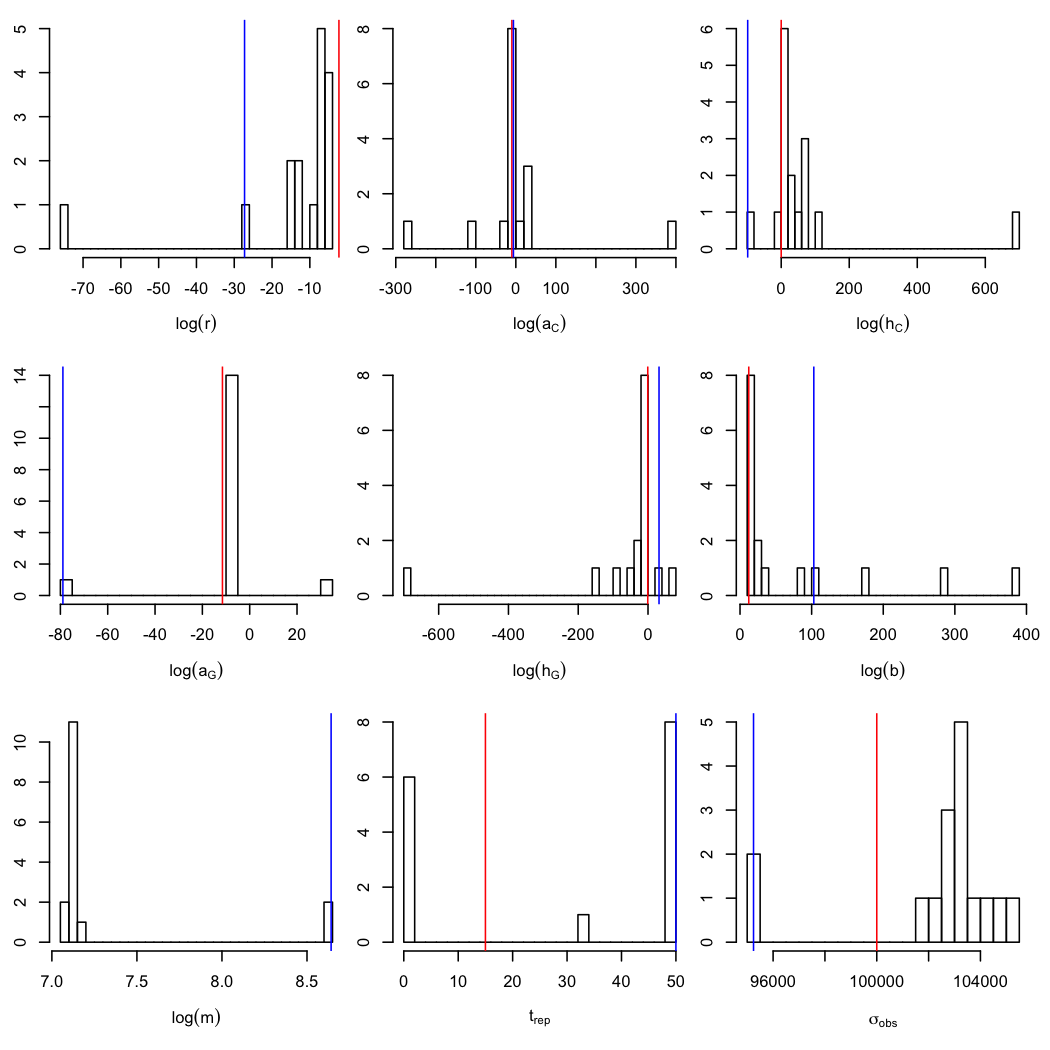
\includegraphics[width=\linewidth]{figure/hist2-1} \hfill{}

\caption[Histograms of parameter estimates for all parameter sets with log-likelihood within 5 units of the best likelihood]{Histograms of parameter estimates for all parameter sets with log-likelihood within 5 units of the best likelihood. The red line shows the true parameter value and the blue shows the parameter value for the set with highest likelihood.}\label{fig:hist2}
\end{figure}


\end{knitrout}

The other issue was whether a simpler model would actually be able to fit the data better than the more complex, data-generating model.
To see that we need to compare the likelihoods of the best-fitting datasets.
However, we want to weight the likelihood differences by the number of parameters: all else equal, a model with more parameters will always be able to fit the data better.
AIC is a handy metric for such a comparison, defined as $2*k - 2\ln L$, where $k$ is the number of parameters and $L$ is the maximum likelihood.
The model with the \emph{minimum} AIC is the preferred one.
Another interesting thing to do is to ask what the likelihood of the \emph{true} parameter values is.



\begin{knitrout}\scriptsize
\definecolor{shadecolor}{rgb}{0.969, 0.969, 0.969}\color{fgcolor}\begin{kframe}
\begin{alltt}
\hlkwd{print}\hlstd{(AICstructured)}
\end{alltt}
\begin{verbatim}
## [1] 2594.641
\end{verbatim}
\begin{alltt}
\hlkwd{print}\hlstd{(AICunstructured)}
\end{alltt}
\begin{verbatim}
## [1] 2600.815
\end{verbatim}
\begin{alltt}
\hlkwd{print}\hlstd{(AICtruth)}
\end{alltt}
\begin{verbatim}
## [1] 2590.27
\end{verbatim}
\end{kframe}
\end{knitrout}

Here you can see that the true parameter values do provide a better fit to the observed data than do either the unstructured or the structured model.
Importantly, however, the structured model outperforms the unstructured model.
This at least gives me some confidence that data only on transmission stages might still provide enough information to support a structured over an unstructured model.

I further checked this by running 40 different parameter sets and looking at the comparison between the best-fit parameter estimates and the truth (Fig. \ref{fig:forty}).
Again, you can see that the parameters are estimated very poorly (very small, $< 10^{-5}$, and very large $>10^{10}$ parameter estimates were dropped).
However, of all of the parameters, the observation error is actually pretty well estimated.

\begin{knitrout}\scriptsize
\definecolor{shadecolor}{rgb}{0.969, 0.969, 0.969}\color{fgcolor}\begin{figure}

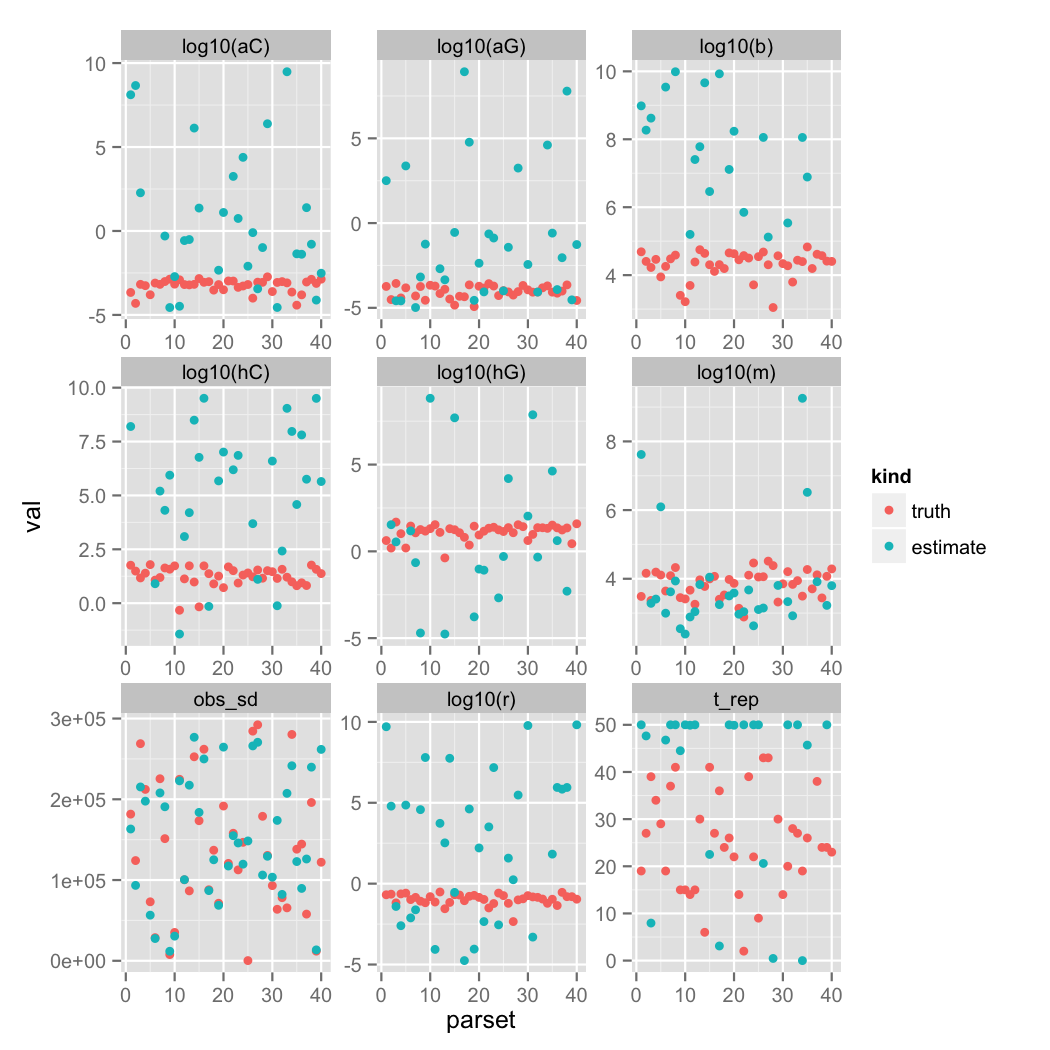
\includegraphics[width=\linewidth]{figure/forty-1} \hfill{}

\caption[Comparison of best-fit estimates to true parameter values across 40 parameter sets]{Comparison of best-fit estimates to true parameter values across 40 parameter sets.}\label{fig:forty}
\end{figure}


\end{knitrout}

Looking at the AIC across these parameter sets (Fig. \ref{fig:aiccomp}), a couple of things jump out.
First is the very small amount of variation in the structured model fits - these are typically very close to one another, suggesting that the fitting has a hard time distinguishing among parameter sets.
The structured models show much wider variation, indicative of the fact that different parameter sets produce very different dynamics.
Second is the fact that, for many parameter sets, the unstructured model has a better fit. In fact, in 35/40 cases, the unstructured model fits better than the structured model.
That suggests that, indeed, it may be hard to estimate the parameters of a structured model.
\begin{knitrout}\scriptsize
\definecolor{shadecolor}{rgb}{0.969, 0.969, 0.969}\color{fgcolor}\begin{figure}

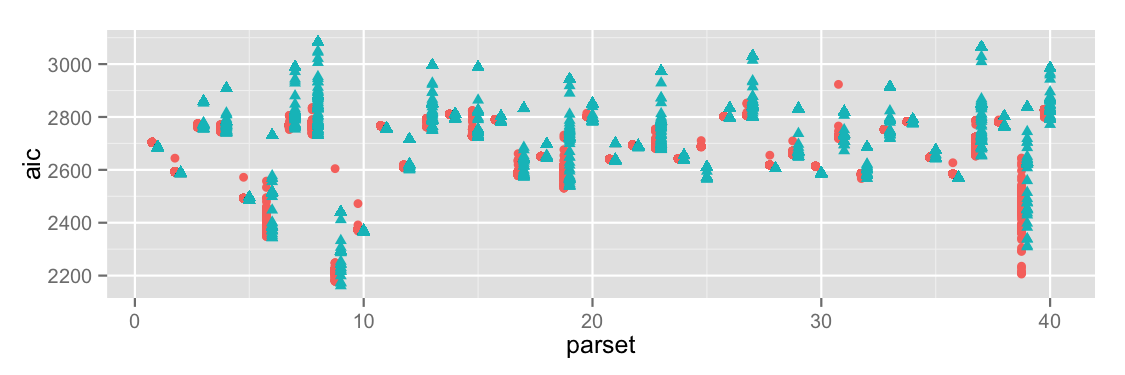
\includegraphics[width=\linewidth]{figure/aiccomp-1} \hfill{}

\caption[Comparison of structured (red) and unstructured (teal) model AIC across 40 parameter sets]{Comparison of structured (red) and unstructured (teal) model AIC across 40 parameter sets. Lower AIC is better here.}\label{fig:aiccomp}
\end{figure}


\end{knitrout}


\clearpage

\section*{Estimating the parameters of a DEB model using simulated data}

Let's begin by laying out the standard dynamic energy budget model, and then discuss ways to include parasitism into that model.
The model begins with the dynamics of ``reserves'', a pool of metabolizable energy that is in temporary storage.
The dynamics of reserves are simple to state, and complicated to derive: the dynamics are just the difference between assimilation rate $p_A$ and mobilization rate $p_C$ (the 'C' is for 'catabolization').
\begin{equation}
\frac{dE}{dt} = p_A - p_C.
\end{equation}
The dynamics of assimilation depend on the feeding model.

Let me begin by basing the feeding model off of Cat's feeding rate data and Spencer's fits.
Cat calculated the clearance rate as $\log(F_0/F_1)*V/T$, where $F_0$ is the initial number of algae cells, $F_1$ is the final number of algae cells, $V$ is the volume of the tube, and $T$ is the duration of the feeding trial (3 hours).
This model assumes an exponential decrease in the number of algae cells, with the rate of decrease determined by the clearance rate of the daphnid; essentially, the daphnid has a linear functional response.
Cat also calculates a size-corrected clearance rate as the observed clearance rate divided by the square of the length, that is, assuming that clearance rate is dependent on the surface area.
Spencer then fit different feeding models to these clearance rate observations, estimating clearance rate parameters, as well as parameters for the dependence of clearance rate on length and spore load.

I actually use a slightly modified version of the standard DEB model that tracks resources in terms of carbon.
Thus, carbon is ingested and assimilated into reserves; carbon that is mobilized out of reserves is used for growth and reproduction, there are no conversion costs, as there are in the standard DEB, for going between reserves, structure, and eggs.
I also do not assume that there is any ``maturity maintenance'' costs; this prevents the possibility of a sexually mature animal ``reverting'' to sexual immaturity.
I am also using Spencer's ingestion model.
In the experiments, although not technically in chemostats, I believe that food was held as close to constant as possible (daily food transfers, saturating food).
The model I am using is:
\begin{align}
\frac{dE}{dt} &= \rho I_{max} L_{obs}^g \epsilon F - p_C,
\frac{dW}{dt} &= \kappa~p_C - k_M~W, \\
\frac{dR}{dt} &= \frac{(1-\kappa)~p_C}{E_R}, \\
p_C &= E \left(\frac{\frac{v}{L} + k_m}{1+\frac{\kappa E}{W}}\right).
\end{align}
A bit of explanation.
Spencer's best-fitting ingestion model for uninfected individuals was $I_{max} L_{obs}^g$, which gives the clearance rate in terms of ml/day, for an individual with observed length $L_{obs}$.
$F$ is the concentration of algal cells in cells/ml; $\epsilon$ is the carbon content of a cell of algae in mgC/cell; $\rho$ is the assimilation efficiency.
$p_C$ is the mobilization rate based on the standard DEB model with $E_G=1$; $\kappa$ is the fraction of carbon allocated towards growth; $k_m$ is the maintenance rate; $E_R$ is the cost of an egg; $v$ is the ``energy conductance''; $L$ is the ``structural length,'' which is not identical to the observed length.
For that matter, $W$ is not the same as the weight you would measure, because the combustion weight would also include $E$, so $W_{obs}=W+E$.
To relate the observed length, we can use published length-weight regressions: $W_{obs} = \xi L_{obs}^q$.

This is the description of the growth dynamic under ``good'' food conditions.
How to deal with starvation is a huge uncertainty in these models.

I am going to use this model for some simulation/recovery experiments.
In particular, I am going to assume that all of the parameters relating to ingestion ($\rho$, $\epsilon$, $I_{max}$, $g$, $F$, $\xi$, and $q$) are known, and focus only on estimating $\kappa$, $k_m$, $E_R$, $v$, and the error in the observation of length.
Even under these circumstances, estimation is a huge challenge.
You can see in Fig. \ref{fig:growth-reprod-1} very clearly that (1) none of the best-fit parameter values are correct (the true values are $\kappa=0.3$, $k_m=0.33$, $E_R=4.27\times10^{-4}$, and $v=5$); (2) the estimates of $\kappa$, $k_m$, and $E_R$ are highly correlated with one another; (3) there is very little signal to detect the value of $v$.
There is some evidence that when $v$ is small, it is also highly correlated with $\kappa$, $k_m$, and $E_R$.

\begin{knitrout}\scriptsize
\definecolor{shadecolor}{rgb}{0.969, 0.969, 0.969}\color{fgcolor}\begin{figure}

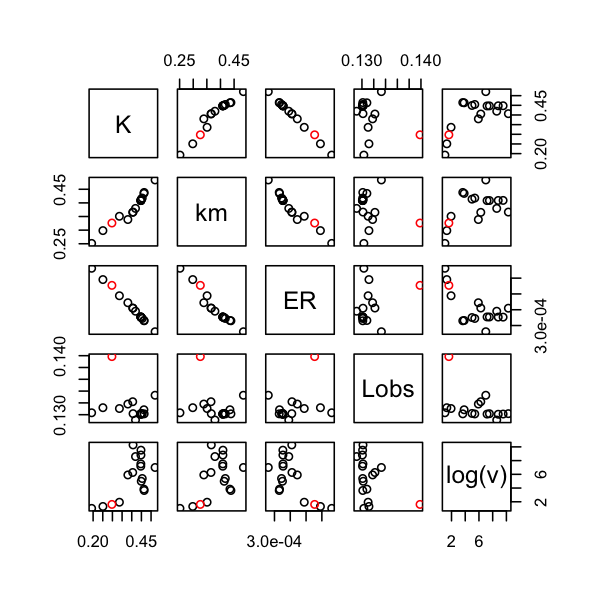
\includegraphics[width=\linewidth]{figure/growth-reprod-1-1} \hfill{}

\caption[Scatterplots showing pairs of parameter estimates for a single parameter set]{Scatterplots showing pairs of parameter estimates for a single parameter set. Only parameter sets within 2 log-likelihood units of the best-fitting parameter set are included. The red points show the true parameter values.}\label{fig:growth-reprod-1}
\end{figure}


\end{knitrout}

The non-identifiability of $v$ is actually somewhat expected.
Martin et al. (2013) found a similar problem, and ended up fixing the value of $v$ and then estimating the other parameters.
You can see from the profile likelihood for $v$ that a huge range of $v$ values are almost equally supported by the data (Fig. \ref{fig:profile-v}).
For this figure, I held all parameters constant at their values when the likelihood was maximized; I then varied $v$ against this background.
Essentially, it appears that $v$ sits along a long ridge in likelihood space.
\begin{knitrout}\scriptsize
\definecolor{shadecolor}{rgb}{0.969, 0.969, 0.969}\color{fgcolor}\begin{figure}

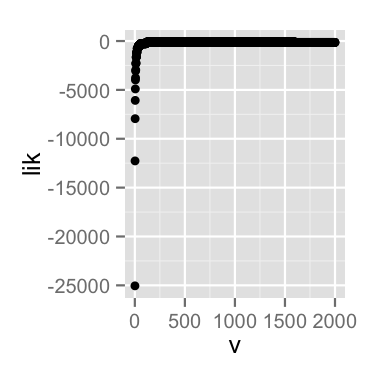
\includegraphics[width=0.6\textwidth]{figure/profile-v-1} \hfill{}

\caption[Profile likelihood for the energy conductance v]{Profile likelihood for the energy conductance v.}\label{fig:profile-v}
\end{figure}


\end{knitrout}

Clearly, estimating $v$ along with the other parameters is impossible in this modeling framework.
The question is how much you can tighten up the estimates of the other parameters by fixing the value of $v$ at something.
To address this, I fixed $v$ at a range of values from 1 to 2000 and fit the other four parameters.
The results of this fitting can be seen in (Fig. \ref{fig:growth-reprod-2}).
Here, for each value of $v$, I plot the parameter estimates for any parameter set within 2 log-likelihood units of the highest likelihood parameter set.
You can see immediately how much the parameter estimates have tightened up: the range of parameter estimates is much smaller.
Moreover, the highest-likelihood parameter set is nearly identical, almost regardless of the value of $v$ (this can be seen from the fact that the best-fitting parameter values form essentially a straight line as $v$ increases).
However, although the estimates are consistent, they are actually not very close to the true parameter values (given in the plot titles).
The estimates do appear to be getting closer for values of $v < 20$.

\begin{knitrout}\scriptsize
\definecolor{shadecolor}{rgb}{0.969, 0.969, 0.969}\color{fgcolor}\begin{figure}

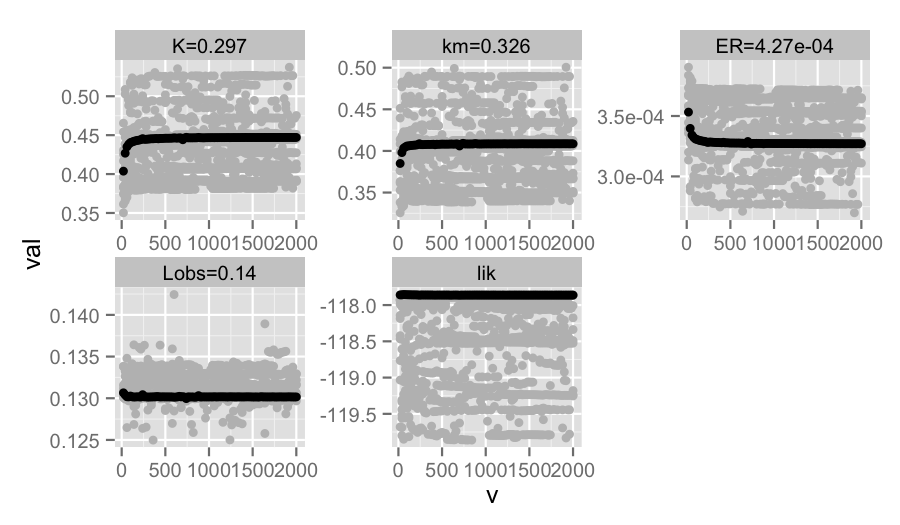
\includegraphics[width=\linewidth]{figure/growth-reprod-2-1} \hfill{}

\caption[Parameter estimates for fixed values of v]{Parameter estimates for fixed values of v. All estimate shown are within 2 log-likelihood units of the best fitting parameter set, which is indicated by black points.}\label{fig:growth-reprod-2}
\end{figure}


\end{knitrout}

Fig. \ref{fig:growth-reprod-3} shows the parameter estimates when $v$ is held towards slightly smaller values.
Interestingly, for $v=5$, the parameter estimates are really close to the true values and the likelihood is essentially maximal.

\begin{knitrout}\scriptsize
\definecolor{shadecolor}{rgb}{0.969, 0.969, 0.969}\color{fgcolor}\begin{figure}

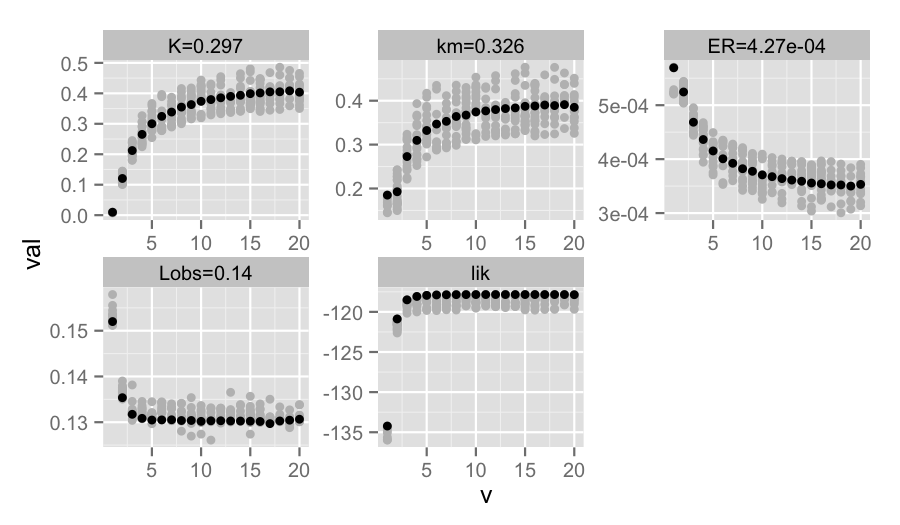
\includegraphics[width=\linewidth]{figure/growth-reprod-3-1} \hfill{}

\caption[Parameter estimates for smaller, fixed values of v]{Parameter estimates for smaller, fixed values of v.}\label{fig:growth-reprod-3}
\end{figure}


\end{knitrout}

If you look very, very closely, you can see that there actually is a peak in the likelihood surface at $v=12$ (Fig. \ref{fig:v-lik-peak}).
Of course, the likelhood difference is less the 3/100 of a log-likelhood unit, or less than 1 likelihood unit.
Such a small difference would likely not be significant, so there is essentially no statistical evidence supporting any particular $v$ value, so long as it is greater than 5 or so.
\begin{knitrout}\scriptsize
\definecolor{shadecolor}{rgb}{0.969, 0.969, 0.969}\color{fgcolor}\begin{figure}

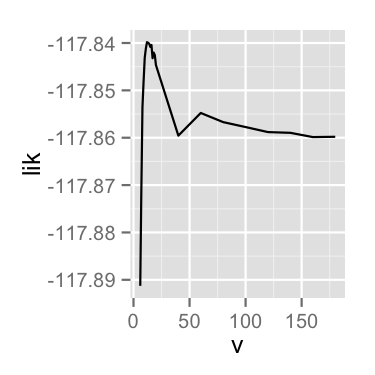
\includegraphics[width=0.6\textwidth]{figure/v-lik-peak-1} \hfill{}

\caption[Very small likelihood peak at low v values]{Very small likelihood peak at low v values.}\label{fig:v-lik-peak}
\end{figure}


\end{knitrout}

I will point out here that a very high value of $v$ essentially creates a ``reserve-less'' DEB model.
In such a model, there is no buffer between the environment and daphnid life history, so growth and reproduction depend directly on ingestion.
This result is not unexpected, as evidenced by the success of net production models (the standard DEB is a net assimilation model) for predicting individual growth and reproduction (Noonburg et al. 1998, Nisbet et al. 2004) and population dynamics (McCauley et al. 2008) of \emph{Daphnia}.
Of course, the high support for a very large value of $v$ might be because I have assumed constant food, rather than a dynamically variable food source.

\clearpage

\section*{Fitting the feeding model}
Let's revisit the actual experimental conditions, which did not hold food constant.
The experimental conditions were as follows:
\begin{itemize}
\item Within the first 24 hours of life, all individuals were placed in 2ml of lake water with 20,000 cells of algae and exposed to parasites.
\item After 24 hours of parasite exposure, animals were moved to beakers with 30ml of water and fed 1,000,000 cells of algae every day.
\item Animals were transferred to clean water every 5 days.
\end{itemize}
The hope was that this is so much food that \emph{D. dentifera} cannot eat it all in a day, so that if the true feeding model is a size-dependent Type II functional response (which it probably is), i.e,
\begin{equation}
I_{max} \frac{F}{f_h+F} L^g,
\end{equation}
then $F$ is so large that it is reasonable to assume that $F/(f_h+F) \approx 1$.

We can make a back of the envelope calculation to see how reasonable this assumption might be.
In particular, let's figure out a reasonable guess for the half-saturation constant $f_h$.
Hall et al. use a value of $f_h = 0.1$ mgC/L based on Nisbet et al. 2004, which is not too far off of the value used by McCauley et al. 1990, 2008 of 0.164 mgC/L.
The concentration of algae added to the beaker each day was $3.33 \times 10^7$ cells/L.
Using an estimate of the carbon content per algal cell (according to Rachel, 20,000 cells contained 0.89ug C) of $4.45 \times 10^{-8}$ mgC/cell, the initial concentration of algae was 1.48 mgC/L.
With this initial concentration, $F/(f_h + F) \approx 0.94$.
This suggests that it might be problematic to assume that food is always high, at least for that first day after feeding.
However, the container was only changed every 5 days, so every time more food was entered, any uneaten food that had settled out would have been resuspended, making it available to the \emph{Daphnia}.
This might make assuming $F/(f_h+F)\approx 1$ a more reasonable assumption.

However, I think it is worth refitting the feeding model, for three reasons.
First, the feeding model parameters were estimated using the converted clearance rate data, rather than the raw algae counts.
I think it makes more sense to fit the raw data.
Second, the true functional response for \emph{Daphnia} is Type II, but the clearance rate calculation is using a Type I functional response.
The assumption of a Type I functional response becomes problematic when dealing with the resuspension of uningested algae, which will lead to very high algal abundances on the day before a transfer.
Third, there is error in both the estimates of both the initial and final algal abundances that I don't think is being accounted for.
So, using the raw algal count data, I want to estimate the parameters of the following system:
\begin{align*}
\frac{dF}{dt} &= -I_{max} \frac{F}{f_h+F} L^g, \\
F(0) &= F_0.
\end{align*}
The parameters that need to be estimated are $I_{max}$, $f_h$, $g$, $F_0$, and the error in the observation of algal abundances $\sigma_F$.
However, I realize that we probably cannot estimate $f_h$ without variation in the initial concentration of algae.
So I will fix the value of $f_h$ and estimate all of other parameters.
I then vary the value of $f_h$ and repeat the fitting.
This separates the problem of estimating $f_h$ from the problems of estimating the other parameters.
However, since the number of parameters of the model do not change, I can use the value of $f_h$ that leads to the maximum likelihood as the estimate of $f_h$.
Fig. \ref{fig:feeding} shows the all the parameter estimates for each value of $f_h$ and the likelihood.
You can see that it is possible to fit the data well for every value of $f_h$ considered, but that the best-fit value of $I_{max}$ scales linearly with increasing $f_h$.
Similarly, the best-fitting value of $g$ also increases as $f_h$ increases.
The range of $g$ esimates includes the value that Spencer estimated (his estimate was 1.3704).
However, the estimate of the the initial algae abundance $F_0$ and the error in estimating algal abundance $\sigma_F$ are both relatively constant across parameters.
Note that right now, I am working with algal concentrations in units of cells/ml.
Thus $f_h$ has units of cells/ml; $I_{max}$ has units of cells per ml per mm$^g$.
Of course, just because many different parameter sets can fit the feeding data equally well does not automatically imply that they will fit the growth and reproduction data equally well.
This is the next step, I think.
I will use a more accurate model of the actual food treatments, with feeding rate parameters fixed at different values (varying $f_h$ and setting $I_{max}$ and $g$ to be the values the maximized the likelihood for the given $f_h$ value).
I will then fit all of the DEB parameters.
Hopefully there will be a clear best-fitting set of parameter values that will identify both the value of $f_h$ and the DEB parameters.

\begin{knitrout}\scriptsize
\definecolor{shadecolor}{rgb}{0.969, 0.969, 0.969}\color{fgcolor}\begin{figure}

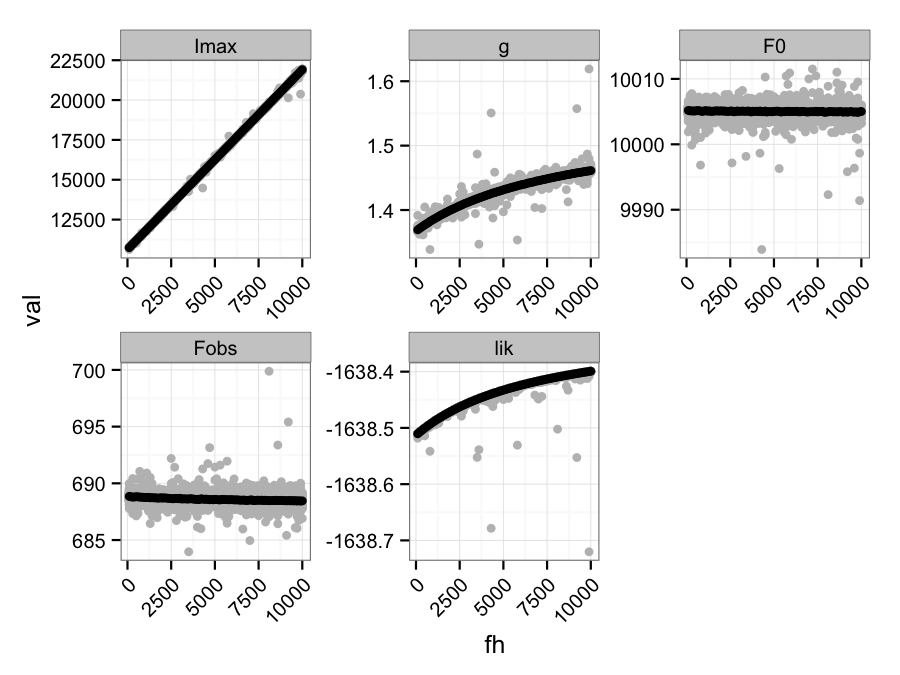
\includegraphics[width=0.8\textwidth]{figure/feeding-1} \hfill{}

\caption[Feeding model parameters for \textbf{uninfected} animals as ]{Feeding model parameters for \textbf{uninfected} animals as $f_h$ is varied. Black points show the maximum likelihood parameter estimates.}\label{fig:feeding}
\end{figure}


\end{knitrout}

But, before I go on, I want to see whether this fitting procedure supports a lower feeding rate for infected \emph{Daphnia}.
As a first pass, I will let all parameters be re-estimated for the uninfected animals, rather than assuming that any of the parameters estimated for the uninfected animals will carry over.
In reality, of course, the initial food abundance and observation error should be the same, at the very least.
Whether $f_h$ and $g$ should also be the same is less clear to me.

Fig. \ref{fig:inf-feeding} shows the results of this feeding.
While $I_{max}$ is definitely much lower for infected animals compared to uninfected animals, the really huge change is the estimates of $g$: whereas $g > 1$ for uninfected animals, for infected animals, feeding rate is nearly independent of size.
This is kind of interesting, actually, although I am not sure what to make of it.
\begin{knitrout}\scriptsize
\definecolor{shadecolor}{rgb}{0.969, 0.969, 0.969}\color{fgcolor}\begin{figure}

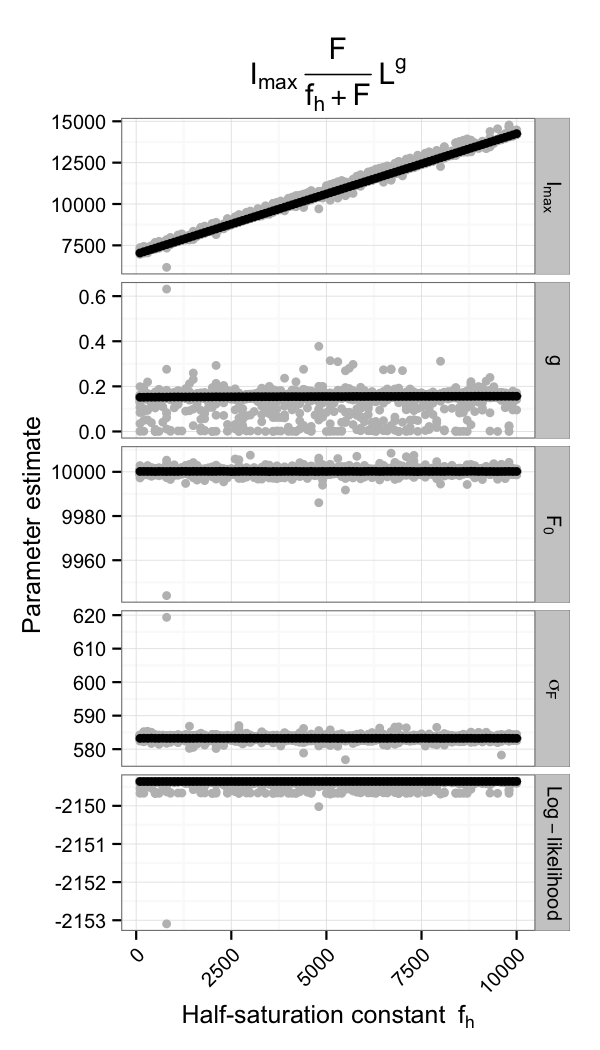
\includegraphics[width=0.8\textwidth]{figure/inf-feeding-1} \hfill{}

\caption[Feeding model parameters for \textbf{infected} animals as ]{Feeding model parameters for \textbf{infected} animals as $f_h$ is varied. Black points show the maximum likelihood parameter estimates for each value of $f_h$.}\label{fig:inf-feeding}
\end{figure}


\end{knitrout}

I also did the fitting fixing $F_0$, $\sigma_F$, and $g$ at the same values as for uninfected animals, so the only parameter I was estimating was $I_{max}$.
In this case, you see an even larger reduction in the estimate of $I_{max}$ between uninfected and infected individuals (Fig. \ref{fig:Imax-comp}).
The likelihood of the $I_{max}$-only model is about 20 log-likelihood units worse than the model where all of the parameters were estimated.
\begin{knitrout}\scriptsize
\definecolor{shadecolor}{rgb}{0.969, 0.969, 0.969}\color{fgcolor}\begin{figure}

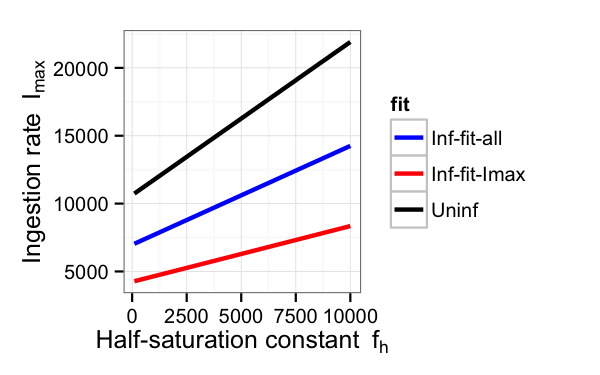
\includegraphics[width=0.7\textwidth]{figure/Imax-comp-1} \hfill{}

\caption[Estimates of ]{Estimates of $I_{max}$ as $f_h$ varies for uninfected animals (black line), for infected animals when all feeding parameters are estimated simultaneously (blue), and for infected animals when $g$ takes the same value as for uninfected animals (red).}\label{fig:Imax-comp}
\end{figure}


\end{knitrout}

Another possibility considered by Spencer is that feeding rate in infected animals is also affected by spore load.
The model he uses, and that I will consider as well, is
\begin{equation*}
\frac{dF}{dt} = -I_{max} \frac{F}{f_h+F} L^g \exp\left(-a\frac{Z}{L^h}\right),
\end{equation*}
where $Z$ is the spore load, $h$ scales body length, and $a$ is the reduction in feeding as the spore load per unit of body size increases.
There is one problem that I don't know how Spencer dealt with, which is how to treat individuals that were exposed but were sacrificed too young to know whether they were infected or not (and were not even checked for spores).
There are two ways to deal with them: either ignore them and only include individuals that were counted, or to treat them all as zeros.
I will try both ways.
(\textbf{Note to self: if I treat these NAs as zeros, I might actually be able to use a structured model.
There are, of course, problems here unless infection success can be assumed to be 100\%.})

For the first attempt, I drop all individuals with NA spore counts.
I estimated $I_{max}$, $a$, and $h$ for a range of $f_h$ values.
I did not attempt to estimate $g$ here, by fixed it at the value estimated for uninfected animals.
The reason for this is that the only infected animals that were counted were fairly large (and thus not growing much).
The lack of variation in size among clearly infected animals makes $g$ nearly impossible to estimate.
Focusing only on parameter sets with log-likelihoods within 1 units of the best-fitting dataset, you can see that the estimates are pretty consistent for a given $f_h$ value (Fig. \ref{fig:spore-dep-feeding}).
Moreover, as $f_h$ increases, the estimates of $a$ and $h$ are basically constant, while $I_{max}$ increases linearly.
The highest likelihood occurs for very small values of $f_h$, though the likelihood difference is small.
The likelihood of this model cannot be compared against the likelihood of the model that did not include spore-dependent feeding reductions because all animals with NA spore counts were dropped here.

\begin{knitrout}\scriptsize
\definecolor{shadecolor}{rgb}{0.969, 0.969, 0.969}\color{fgcolor}\begin{figure}

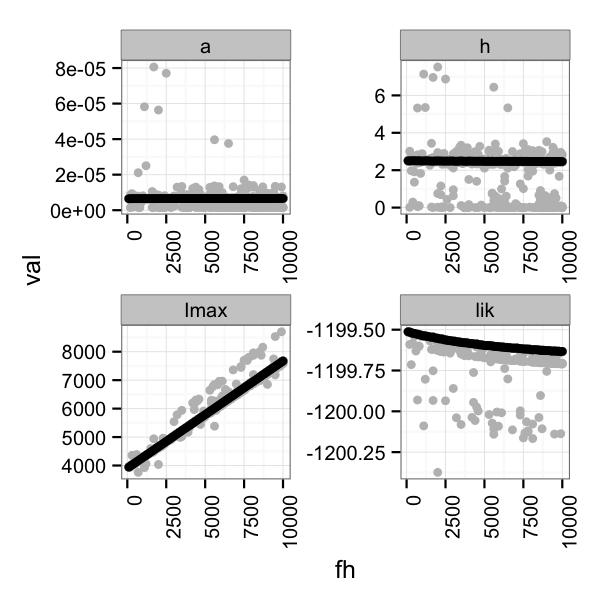
\includegraphics[width=0.8\textwidth]{figure/spore-dep-feeding-1} \hfill{}

\caption[Spore-dependent feeding model parameters for infected animals as ]{Spore-dependent feeding model parameters for infected animals as $f_h$ is varied. Black points show the maximum likelihood parameter estimates for each value of $f_h$. For this fitting, all individuals with NA spore counts were dropped.}\label{fig:spore-dep-feeding}
\end{figure}


\end{knitrout}

If I treat all of the young exposed individuals as infected, but with 0 spore counts instead, the results are quite different.
Comparing Figs. \ref{fig:spore-dep-feeding} and \ref{fig:spore-dep-feeding-2}, you can see that all three parameters ($a$, $h$, and $I_{max}$ increase in value quite a lot when you assume that all of the individuals with NA spore counts are actually infected and have 0 transmission stage spores.
However, although the best-fitting parameter sets have the same values of $a$ and $h$ as $f_h$ increases, there is much more spread around each estimate.
That is, a much greater range of parameter values have nearly equal likelihoods.
That said, I think, in the end, that the parameter estimates shown in Fig. \ref{fig:spore-dep-feeding-2} are the better ones to use.
This is because $Z$ is only considering mature transmission spores, so if you assume that all of the young animals are infected but with 0 transmission spores, then this is the right thing to do.
It also seems reasonable to assume 100\% infection success, given that all of the exposed animals that were sacrificed after day 12 were infected.

\begin{knitrout}\scriptsize
\definecolor{shadecolor}{rgb}{0.969, 0.969, 0.969}\color{fgcolor}\begin{figure}

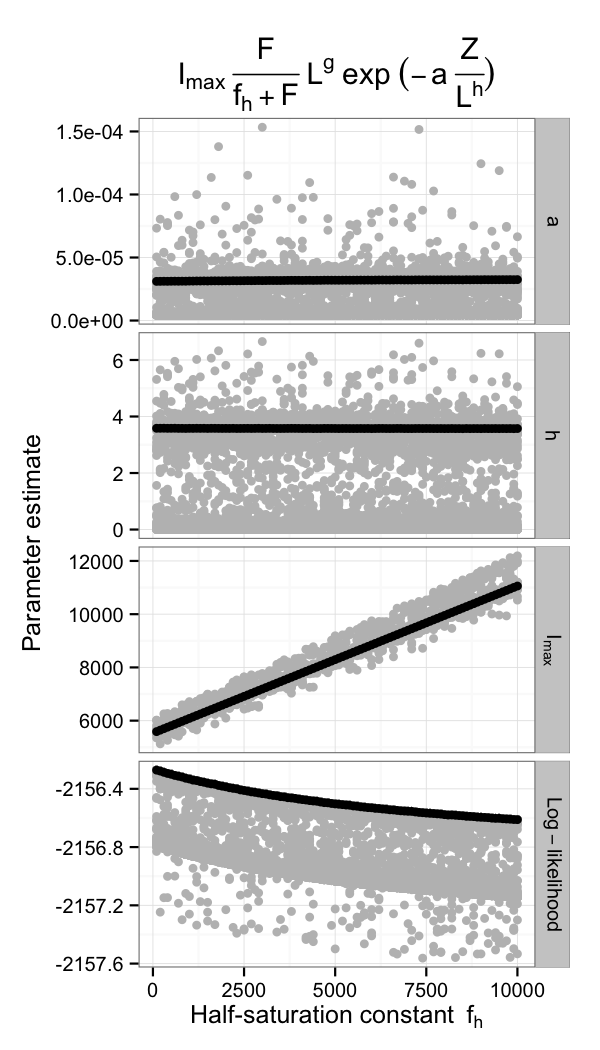
\includegraphics[width=0.8\textwidth]{figure/spore-dep-feeding-2-1} \hfill{}

\caption[Spore-dependent feeding model parameters for infected animals as ]{Spore-dependent feeding model parameters for infected animals as $f_h$ is varied. For this fitting, all individuals with NA spore counts were assumed to have a spore count of 0. Black points show the maximum likelihood parameter estimates for each value of $f_h$.}\label{fig:spore-dep-feeding-2}
\end{figure}


\end{knitrout}

The issue is whether this spore-dependent feeding model has a significantly higher likelihood than the simpler model than assumed spore-independent feeding (the model that fit only $I_{max}$), since that model was also fitted to the data for all exposed individuals.
The likelihood of the spore-dependent model is higher, of course, because there are more free parameters.
Based on AIC$_{\text{c}}$ differences, the spore-dependent model is preferred over the spore-independent model: the AIC$_{\text{c}}$ of the spore-dependent model is 16 units smaller than the AIC$_{\text{c}}$ of the spore-independent model, suggesting that the spore-independent model is about 0.0002 times as probable as the spore-dependent model.
This conclusion is also supported by a likelihood ratio test, which suggests that the probability of such a likelihood difference occurring by chance as less than $10^{-4}$.



I can also compare the observed data against model predictions for both infected and uninfected animals.

In particular, I will calculate the expected clearance rate for every animal, based on the best-fitting model (assuming $f_h = 5000$), and compare that prediction against the observed clearance rate.
For this model, the parameter estimates were $g=1.43$, $a=3.2\times10^{-5}$, and $h=3.56$, with $I_{max}=16264$ for uninfected animals and $I_{max}=8293$ for infected animals.
Clearance rate was calculated as $\log\left(\frac{F(0)}{F(t)}\right)~\frac{V}{t}$, where $V$ is the volume of beaker, $t$ is the total time of the trial, and $F(0)$ and $F(t)$ give the concentration of food at time 0 and time $t$, respectively.
Fig. \ref{fig:clearance-thru-time} shows how clearance rate changes across the age of the individuals.
You can see clearly that infected animals feed at a lower rate than uninfected animals.
The model tends to underpredict feeding rate early in life for both sick and healthy animals, and the variance in the expected feeding rate among animals of the same age is much smaller than the observed variance.
However, the predicted variance is higher than what is observed here because I am not taking account of the observation error - I could have plotted error bars around each of the predicted points based on the observation error in both initial and final food concentrations.

\begin{knitrout}\scriptsize
\definecolor{shadecolor}{rgb}{0.969, 0.969, 0.969}\color{fgcolor}\begin{figure}

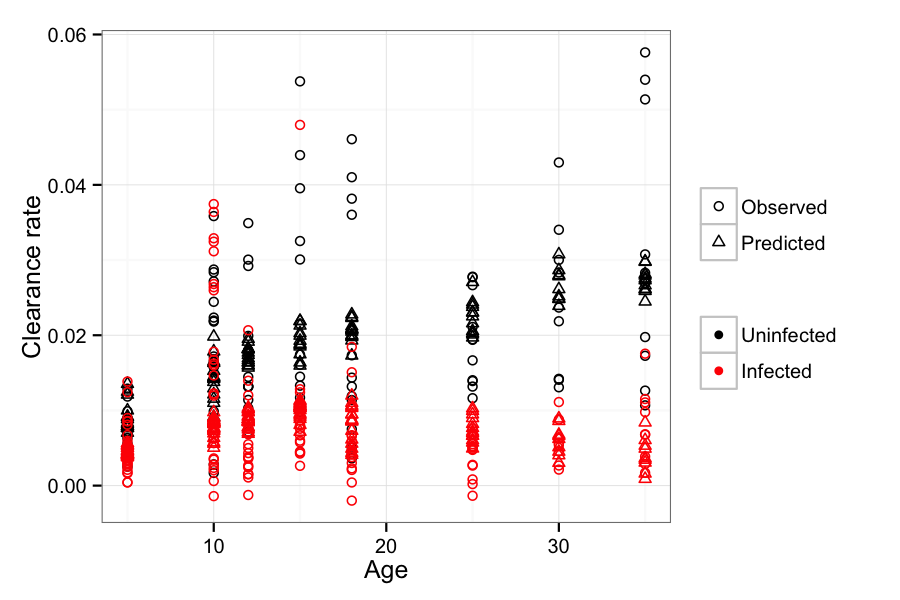
\includegraphics[width=\linewidth]{figure/clearance-thru-time-1} \hfill{}

\caption[Comparing observed versus predicted clearance rates for both infected and uninfected animals across the lifespan, assuming the best fit parameter values]{Comparing observed versus predicted clearance rates for both infected and uninfected animals across the lifespan, assuming the best fit parameter values.}\label{fig:clearance-thru-time}
\end{figure}


\end{knitrout}

The last thing that I want to do is to see if my feeding model does a better job fitting the data than does the parameter estimates reported by Spencer.
Let's hope so, since I spent so much time fitting the data!
To evaluate this, I will plot the observed versus predicted clearance rates for each individual and then calculate an $R^2$ value based on the difference between each individual datapoint and the one-to-one line.
I will do this for my model, and also for Spencer's model, which predicted the clearance rates as
\begin{align}
f_U~L^g & \text{for uninfected animals}, \\
f_I~L^g~\exp\left(-a~\frac{Z}{L^h}\right) & \text{for infected animals},
\end{align}
with $f_u = 0.0126$, $g=1.3704$, $f_i=0.0061$, $a=0.0205$, and $h=2.6420$.
What you notice right away from Fig. \ref{fig:Clay-vs-Spencer} is that the predicted clearance rate is zero for many of the infected animals, under Spencer's model.
This is because the estimate of $a$ that Spencer reports is much, much higher than my estimate (0.0205 vs. $3.2\times10^{-5}$).
Because of this, the $R^2$ for my model is much higher than Spencer's, 0.36 versus 0.28.
If you focus only on the uninfected animals, our models are equally good (0.257 for my model versus 0.258 for Spencer's model).
Thus, I feel confident moving forward with my model for feeding, with the caveat that I still don't know what the appropriate value of $f_h$ is.
To address this, I will fit growth and reproduction trajectories, with algae having their own dynamics, to see whether this helps at all with tightening up the estimates of both $f_h$ and also $v$, the energy conductance.
I will begin with generating simulated datasets, as before, and fitting the DEB models to those datasets.
It is my hope that the dynamic food resource will reveal both the value of $f_h$ (because algal abundance will drop low enough for it to matter) and $v$ (because dynamic food will cause more dynamism in the value of $E$, thereby making the value of $v$ more important).

\begin{knitrout}\scriptsize
\definecolor{shadecolor}{rgb}{0.969, 0.969, 0.969}\color{fgcolor}\begin{figure}

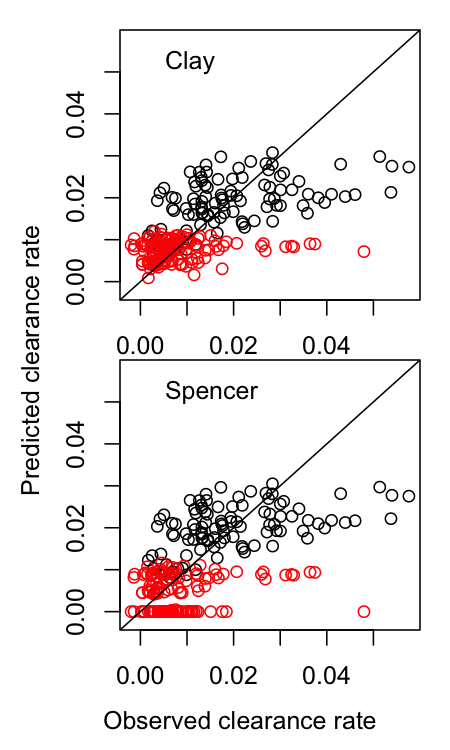
\includegraphics[width=0.6\textwidth]{figure/Clay-vs-Spencer-1} \hfill{}

\caption[Comparing the fits of my model to Spencer's model by plotting observed clearance rates against model-predicted clearance rates for both uninfected and infected animals]{Comparing the fits of my model to Spencer's model by plotting observed clearance rates against model-predicted clearance rates for both uninfected and infected animals.}\label{fig:Clay-vs-Spencer}
\end{figure}


\end{knitrout}

\clearpage
\section*{DEB fitting with dynamic algae}
To begin, I am going to do some simulation/recovery experiments with a DEB model with a dynamically varying resource.
The model I am going to start with is the following:
\begin{align}
\frac{dF}{dt} &= -I_{max} \frac{F}{f_h+F} L_{obs}^g \\
\frac{dE}{dt} &= \rho \epsilon V I_{max} \frac{F}{f_h+F} L_{obs}^g - p_C,
\frac{dW}{dt} &= \kappa~p_C - k_M~W, \\
\frac{dR}{dt} &= \frac{(1-\kappa)~p_C}{E_R}, \\
p_C &= E \left(\frac{\frac{v}{L} + k_m}{1+\frac{\kappa E}{W}}\right).
\end{align}
This model makes the simplifying assumption that the algae are not reproducing.
I will deal with that problem next.
However, I will assume that an amount of food $F_{a}$ is added every day, and that every fifth day the food is reset to $F_{a}$, corresponding to the transfer of the animal to a clean beaker.
The parameters of the feeding model are specified by the best-fitting model above.
However, this model tracks the dynamics of the concentration of algae in cells/ml; to get the total amount of carbon assimilated by the daphnid, I simply multiply the ingestion by $\rho$, the assimilation efficiency, $\epsilon$, the carbon content per cell, and $V$, the total volume of the container.

I performed a quick simulation study to see how well the model was able to recover the parameter estimates.
I simulated a dataset assuming $I_{max}=22500$, $f_h=10000$, $g=1.45$, $\rho=0.1$, $\epsilon = 44.5\times10^{-9}$, $V=30$, $\kappa=0.3$, $k_m=0.15$, $E_R=0.00151$, $v=10$, and a normally distributed observation error standard deviation of $\sigma_L=0.1$.
I attempted to estimate only $\kappa$, $k_m$, $E_R$, $v$, and $\sigma_L$.
You can see from Fig. \ref{fig:dyn-food-hist} that, with the exception of $v$, the parameters were actually fairly well estimated.
Moreover, if you actually look at the log-likelihoods of the best-fitting parameter set and the true parameter set, you find that the best-fitting parameters are actually better than the truth, with the best-fit parameters having a log-likelihood of -90.5 compared to a negative log-likelihood of -91.2 (this is a not-uncommon finding, and it strongly suggests that the fitting algorithm really is honing in).

\begin{knitrout}\scriptsize
\definecolor{shadecolor}{rgb}{0.969, 0.969, 0.969}\color{fgcolor}\begin{figure}

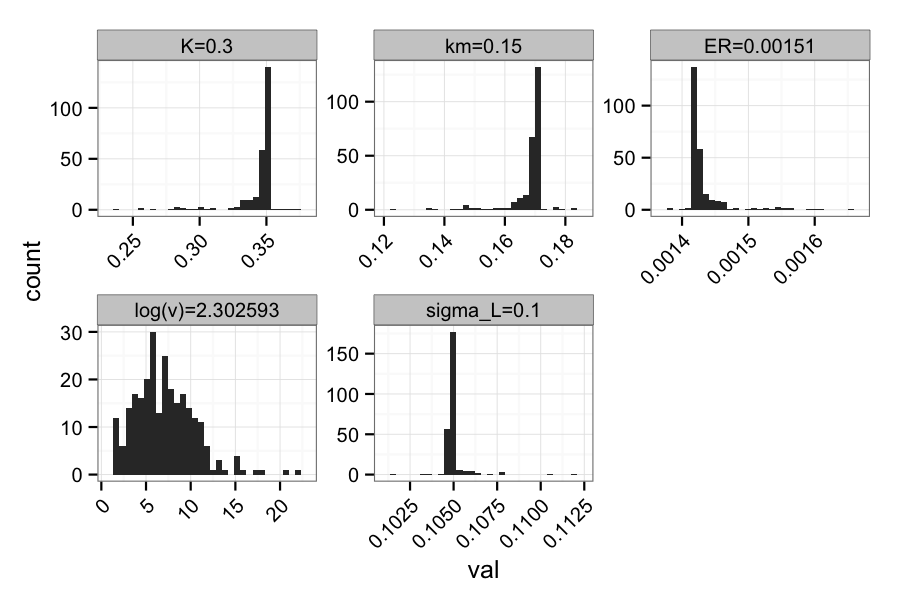
\includegraphics[width=\linewidth]{figure/dyn-food-hist-1} \hfill{}

\caption[Parameter estimates when food is dynamic]{Parameter estimates when food is dynamic.}\label{fig:dyn-food-hist}
\end{figure}


\end{knitrout}

If you construct the profile likelihood for $v$ by fixing it at different values and fitting all of the other parameters, you can see that many values of $v$ are equally supported by the data (Fig. \ref{fig:dyn-food-prof-lik-v}).
As in Fig. \ref{fig:growth-reprod-3}, the parameter estimates are closer to the truth when $v$ is fixed at smaller values.
\begin{knitrout}\scriptsize
\definecolor{shadecolor}{rgb}{0.969, 0.969, 0.969}\color{fgcolor}\begin{figure}

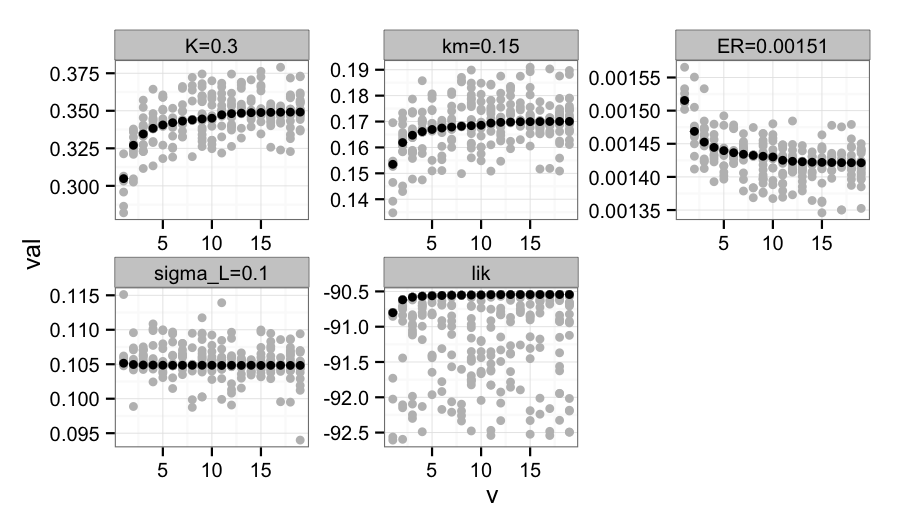
\includegraphics[width=\linewidth]{figure/dyn-food-prof-lik-v-1} \hfill{}

\caption[DEB parameters under dynamic food, when ]{DEB parameters under dynamic food, when $v$ is fixed at different values.}\label{fig:dyn-food-prof-lik-v}
\end{figure}


\end{knitrout}

I am also interested in whether $f_h$ can be estimated on the basis of growth and reproduction data.
For this simulation-recovery experiment, I again fixed $v$ at different values and then attempted to estimate $f_h$ along with $\kappa$, $k_m$, $E_R$, and $\sigma_L$.
During the fitting, as different values of $f_h$ were investigated, the values of $I_{max}$ and $g$ were set at the values that maximized the likelihood based on fitting the feeding data (Fig. \ref{fig:feeding}) - this should deal with the fact that many different values of $f_h$ could fit the feeding data equally well.
For any fixed value of $v$, a large range of $f_h$ values are nearly equally well-supported, and the value of all of the other DEB parameters scales with the value of $f_h$ (Fig. \ref{fig:dyn-food-pairwise}).
There is a peak in the likelihood surface at intermediate $f_h$, which is encouraging, as this peak is actually fairly close to the true value of $f_h$.
The best-fit parameter value is shown by the blue point, and the true value is shown by the red point, so, again, all of the parameters are slightly mis-estimated, but this is probably to be expected.
I still have good evidence that the model can be recovered reasonably well, which is, in an of itself, pretty encouraging.

\begin{knitrout}\scriptsize
\definecolor{shadecolor}{rgb}{0.969, 0.969, 0.969}\color{fgcolor}\begin{figure}

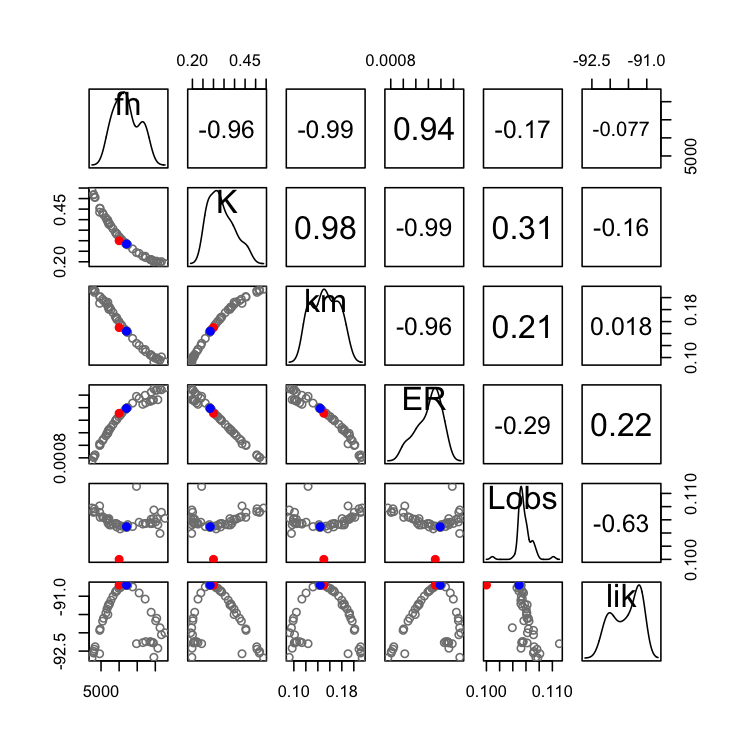
\includegraphics[width=\linewidth]{figure/dyn-food-pairwise-1} \hfill{}

\caption[Pairwise scatterplot of estimates of ]{Pairwise scatterplot of estimates of $f_h$ and DEB parameters when $v=10$.}\label{fig:dyn-food-pairwise}
\end{figure}


\end{knitrout}

We can also look at only the best-fitting parameter set across a range of $v$ values to see how the best-fitting estimate of $f_h$ (and hence the other parameters) depends on the fixed value of $v$.
Fig. \ref{fig:dyn-food-fh-est-profile-v} shows all of the parameter estimates within 2 log-likelihood units of the maximum, for different fixed values of $v$.
Again, you can see that a large number of $f_h$ values are reasonably well supported, driving a lot of variation in the other estimates.
Still, however, the estimate of $f_h$ is reasonably good, and smaller values of $v$, though they have lower likelihoods, produce better estimates of the DEB parameters (though worse estimates of $f_h$).

\begin{knitrout}\scriptsize
\definecolor{shadecolor}{rgb}{0.969, 0.969, 0.969}\color{fgcolor}\begin{figure}

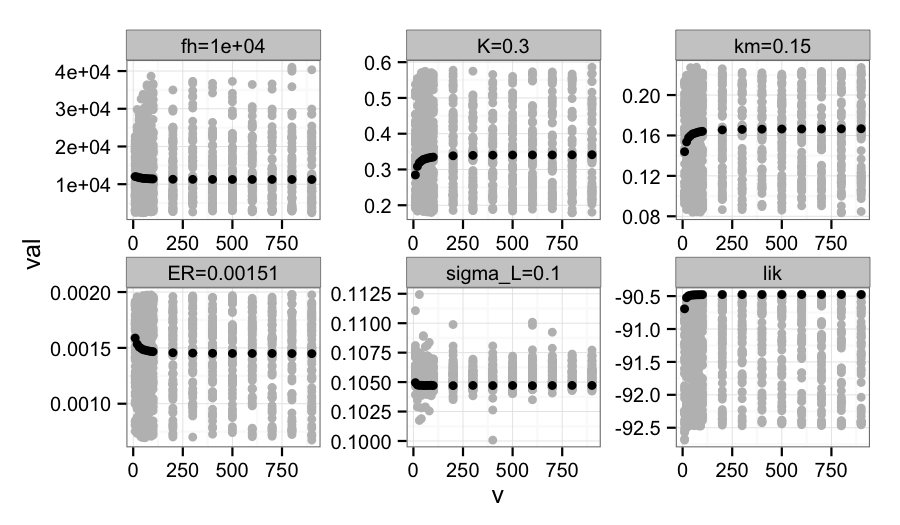
\includegraphics[width=\linewidth]{figure/dyn-food-fh-est-profile-v-1} \hfill{}

\caption[Estimates of ]{Estimates of $f_h$ and the DEB parmaeters as $v$ is varied.}\label{fig:dyn-food-fh-est-profile-v}
\end{figure}


\end{knitrout}

I have left aside one fitting problem till now: estimating $\rho$.
I have the distinct feeling that assimilation efficiency will be almost impossible to estimate, as there will be ways to jigger the other parameters to get equally good fits with almost any value of $\rho$.
To investigate this, I fixed the value of $v=100$ and tried to estimate the DEB parameters, along with $\rho$ and $f_h$.
Fig. \ref{fig:estimating-rho} shows these difficulties.
The estimates of $\rho$ range between 0.2 and 1, with the majority of estimates being very near 1.
There are also clear correlationshp between the estimates of $\rho$ and $\kappa$ and $E_R$, in particular.
These make sense: as assimilation efficiency increases, $\kappa$ must decrease to keep size reasonable; but as $\kappa$ decreases, the cost of reproduction must increase to keep the total egg production reasonable.
The estimates of  $f_h$, $k_m$, and $\sigma_L$ are all still centered near their true values, with likelihood peaks at those values.

\begin{knitrout}\scriptsize
\definecolor{shadecolor}{rgb}{0.969, 0.969, 0.969}\color{fgcolor}\begin{figure}


\includegraphics[width=\linewidth]{figure/estimating-rho-1} \hfill{}

\caption[Scatterplot of parameter estimates when ]{Scatterplot of parameter estimates when $
ho$ is estimated along with $f_h$ and the other DEB parameters. $v$ was fixed at $v=100$ for this estimation.}\label{fig:estimating-rho}
\end{figure}


\end{knitrout}

To further determine how big of a problem estimating $\rho$ is, I did the same kind of profile likelihood calculation, fixing $\rho$ at values between 0.1 and 0.9 and estimating all of the other parameters.
You can see that the fixed value of $\rho$ drives the estimates of $\kappa$ and $E_R$, as before, and that $f_h$, $k_m$, $\sigma_L$ are all reasonably estimated (Fig. \ref{fig:rho-profile}).
More problematically, however, the likelihood increases with increasing values of $\rho$, even though the true value of $\rho$ was 0.1.
This certainly supports my supposition that $\rho$ is very hard to estimate.

\begin{knitrout}\scriptsize
\definecolor{shadecolor}{rgb}{0.969, 0.969, 0.969}\color{fgcolor}\begin{figure}

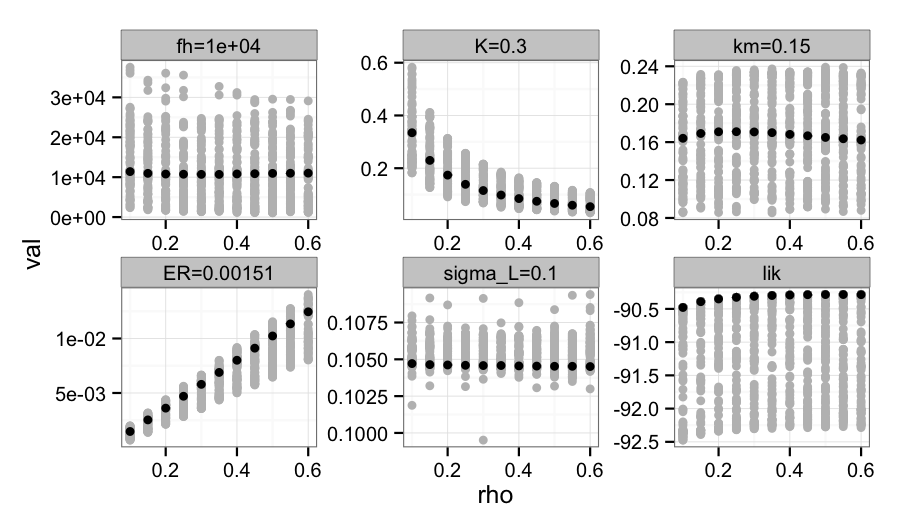
\includegraphics[width=\linewidth]{figure/rho-profile-1} \hfill{}

\caption[Estimates of ]{Estimates of $f_h$ and DEB parameters for different fixed values of $
ho$. For these $v$ was fixed at $v=100$ since there is no evidence so far that the value of that parameter affects the other parameter estimates.}\label{fig:rho-profile}
\end{figure}


\end{knitrout}

However, the strong linear relationship between the fixed value of $\rho$ and the maximum likelihood estimate of $E_R$ suggests a way to estimate $\rho$:
if the value of $E_R$ could be fixed, rather than estimated, that should much more greatly constrain the value of $\rho$.
And, fortunately, $E_R$ is a parameter that is likely plausibly estimated based on the size (and thus, carbon content) of a newborn daphnid.
With that in mind, I redid the fitting, assuming that $E_R = 1.51\times10^{-3}$, the true value in the simulated dataset.
Fig. \ref{fig:est-rho-fix-ER} shows pairwise scatterplots of the parameter estimates when $E_R$ is fixed at its true value and $v$ is fixed at 1000.
You can see from the density plots along the diagonal that the bulk of the estimates are, indeed, close to the true values ($f_h=10000$, $\rho=0.1$, $\kappa=0.3$, $k_m=0.15$, $\sigma_L=0.1$), and that these values correspond to peaks on the likelihood surface.
\begin{knitrout}\scriptsize
\definecolor{shadecolor}{rgb}{0.969, 0.969, 0.969}\color{fgcolor}\begin{figure}


\includegraphics[width=\linewidth]{figure/est-rho-fix-ER-1} \hfill{}

\caption[Parameter estimates when ]{Parameter estimates when $E_R$ is fixed at the true value and $v=1000$.}\label{fig:est-rho-fix-ER}
\end{figure}


\end{knitrout}

If you look across a range of fixed $v$ values, the best-fitting parameter estimates also seem to hone right in on parameter estimates that are close to the true values (Fig. \ref{fig:profile-lik-v-estimating-rho}; the black points show the parameter estimate with highest likelihood).
In particular, the estimates of $\rho$ are quite good.

\begin{knitrout}\scriptsize
\definecolor{shadecolor}{rgb}{0.969, 0.969, 0.969}\color{fgcolor}\begin{figure}

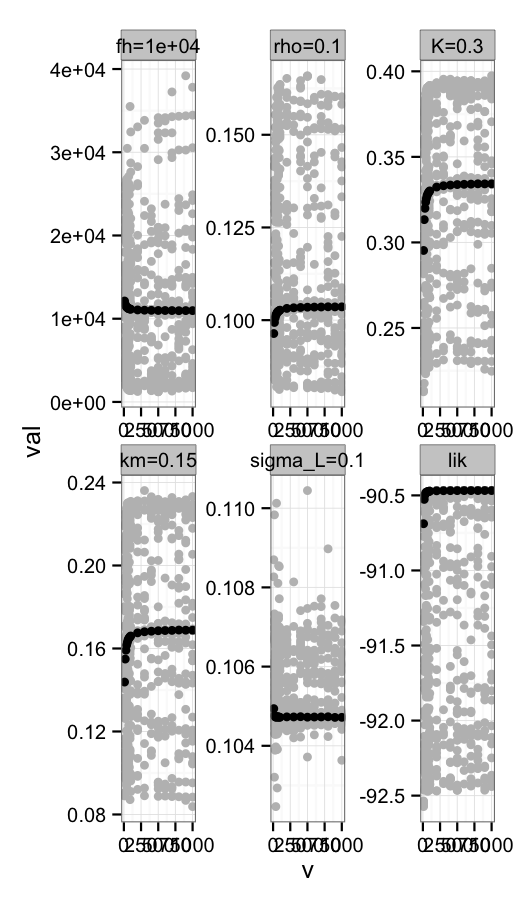
\includegraphics[width=\linewidth]{figure/profile-lik-v-estimating-rho-1} \hfill{}

\caption[Estimates of DEB parameters across a range of ]{Estimates of DEB parameters across a range of $v$ values, when $E_R$ is fixed at its true value.}\label{fig:profile-lik-v-estimating-rho}
\end{figure}


\end{knitrout}

Okay, all of the preceding has been based on fitting a single dataset, and hence a single parameter set.
The last thing to do before moving on to deal with the real data is to simulate datasets with a much wider range of parameter values and attempt to fit those datasets as well.
For this, I generated 20 simulated datasets.
There were some constraints on the parameters and the simulated datasets, to ensure they were somewhat biologically realistic for \emph{Daphnia}.
In particular, all of the parameters had to be positive and $\rho$ and $\kappa$ had to be between 0.1 and 0.9.
I also only accepted parameter sets that produced simulated data such that the observed length at day 5 was less than 2 mm and the observed egg production was 0; moreover, the length at day 35 had to be between 0.5 and 4mm and the egg production at day 35 had to between 5 and 200 eggs.
Finally, some growth had to be observable in the data (a linear regression of length against time had to have a significantly positive slope).
These are fairly tame restrictions; Fig. \ref{fig:sim-datasets} shows smoothed fits of the growth and reproduction data through time to show the variability in growth and reproduction trajectories across the datasets.

\begin{knitrout}\scriptsize
\definecolor{shadecolor}{rgb}{0.969, 0.969, 0.969}\color{fgcolor}\begin{figure}

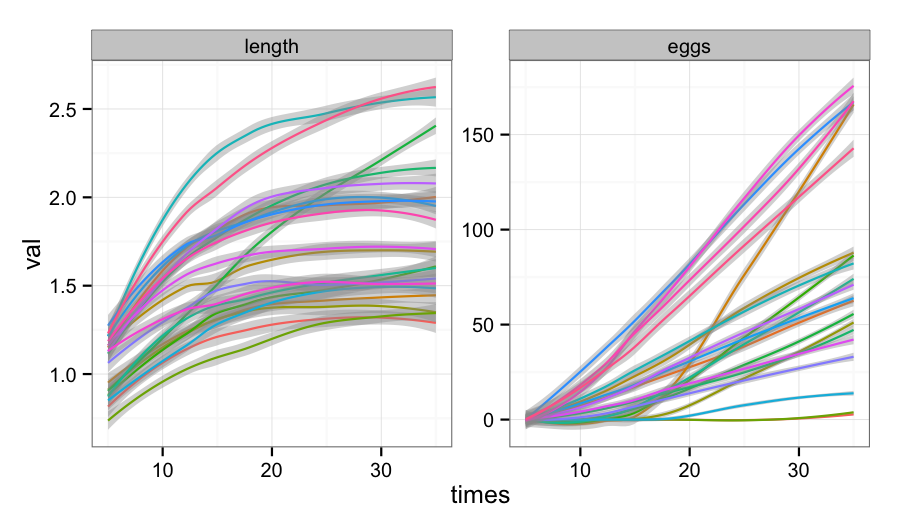
\includegraphics[width=\linewidth]{figure/sim-datasets-1} \hfill{}

\caption[Growth and reproduction trajectories across the 20 simulated datasets]{Growth and reproduction trajectories across the 20 simulated datasets. What is shown is not the raw data, but a smoothed fit of that data. This cleans up the figures but still shows the variability among datasets.}\label{fig:sim-datasets}
\end{figure}


\end{knitrout}

Fig. \ref{fig:mult-datasets-fitting} plots the results of the fitting.
For every parameter set (1-20), I plot all of the parameter estimates that were within 2 log-likelihood units of the best-fitting parameter set.
The parameter set with highest likelihood is shown in black.
The true parameter value is shown in red.
You can see that the overall message here is really encouraging - the best-fitting parameter estimates are typically quite close to the true values.
The exception is certainly with a few of the estimates of $f_h$ (e.g., datasets 10 and 12).
Some datasets also elicited a lot more variability in the parameter estimates that were near the highest likelihood (e.g., dataset 18).
The estimates of $k_m$ were the most variable

\begin{knitrout}\scriptsize
\definecolor{shadecolor}{rgb}{0.969, 0.969, 0.969}\color{fgcolor}\begin{figure}

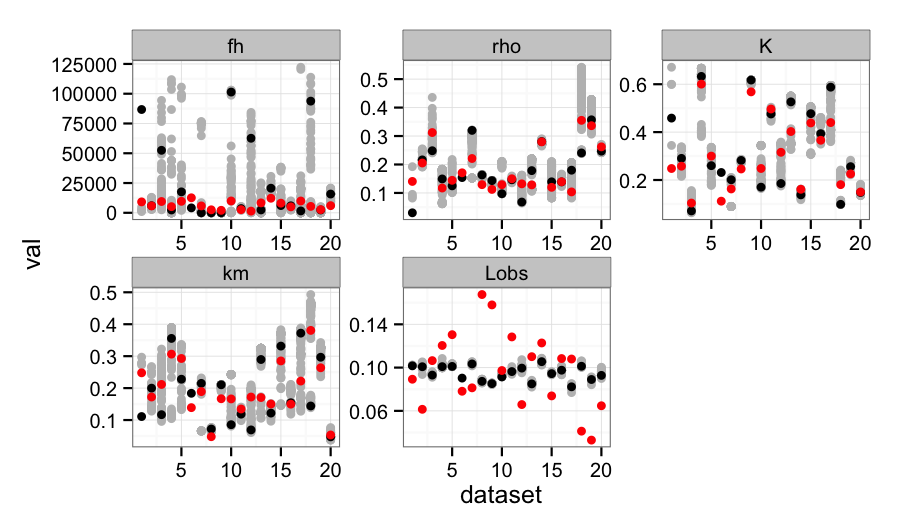
\includegraphics[width=\linewidth]{figure/mult-datasets-fitting-1} \hfill{}

\caption[Parameter estimates across 20 different parameter sets]{Parameter estimates across 20 different parameter sets. The black point shows the best-fitting parameter estimate. The grey points are parameter estimates within 2 log-likelihood units of the best. The red point is the true parameter value. For these fits, $v$ was fixed at 100.}\label{fig:mult-datasets-fitting}
\end{figure}


\end{knitrout}

An examination of the plots of the likelihood against the parameter estimates can help to understand when the parameter estimates were close the true parameter values.
Fig. \ref{fig:lik-against-ests-1} shows some likelihood surfaces when the parameter estimates were quite close to the truth (similar surfaces were revealed for other datasets that were well-estimated (datasets 3, 15, 16, 17, and 20).
Here you can see a single, well-defined likelihood peak.
In this case, the best-fitting parameter estimate (shown by the vertical green line) is quite close to the true parameter estimate (shown by the vertical red line).

\begin{knitrout}\scriptsize
\definecolor{shadecolor}{rgb}{0.969, 0.969, 0.969}\color{fgcolor}\begin{figure}

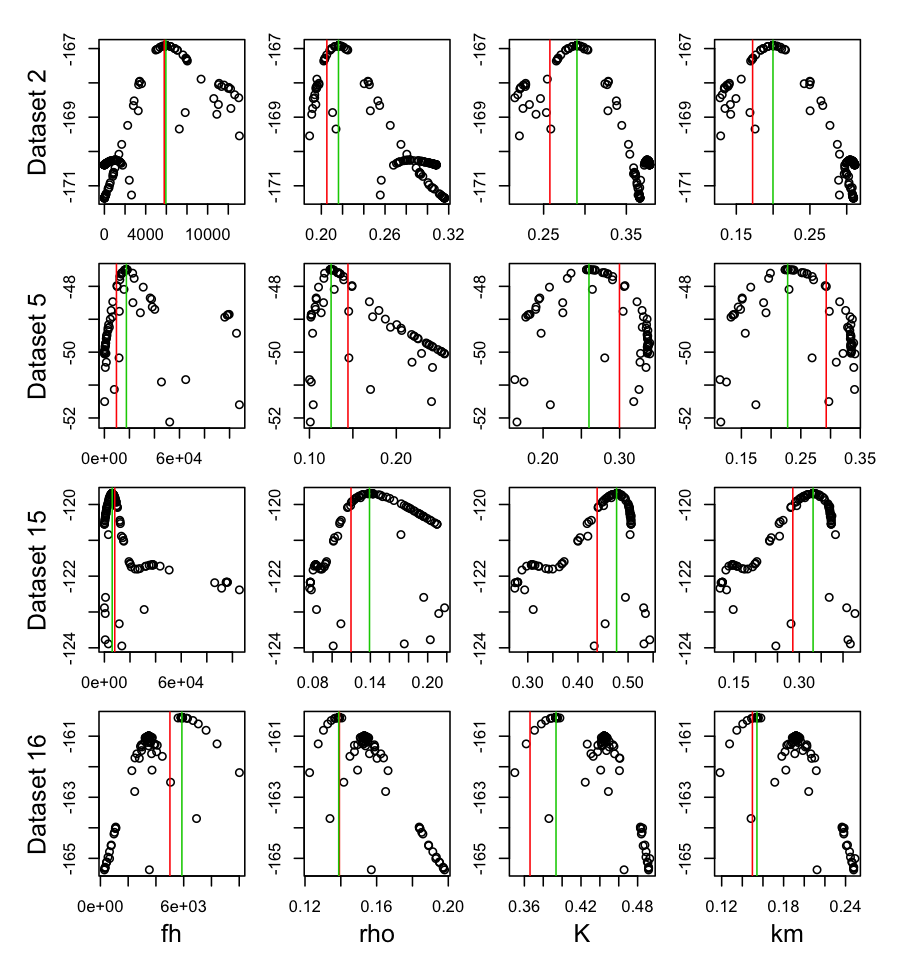
\includegraphics[width=\linewidth]{figure/lik-against-ests-1-1} \hfill{}

\caption[Plots of the likelihood against the parameter estimates for many of the datasets reveals a single likelihood peak, and most of the parameter estimates are quite close]{Plots of the likelihood against the parameter estimates for many of the datasets reveals a single likelihood peak, and most of the parameter estimates are quite close.}\label{fig:lik-against-ests-1}
\end{figure}


\end{knitrout}

On the other hand, Fig. \ref{fig:lik-against-ests-2} reveals that, for some of the datasets where the parameter estimates were further from the truth, the likelihood surface has multiple peaks.
In all of these cases, one of the likelihood peaks is centered around a high $f_h$ value.
In Fig. \ref{fig:lik-against-ests-2}, the likelihood is higher at this large $f_h$ peak, pulling all of the other parameter estimates away from their true values.

\begin{knitrout}\scriptsize
\definecolor{shadecolor}{rgb}{0.969, 0.969, 0.969}\color{fgcolor}\begin{figure}

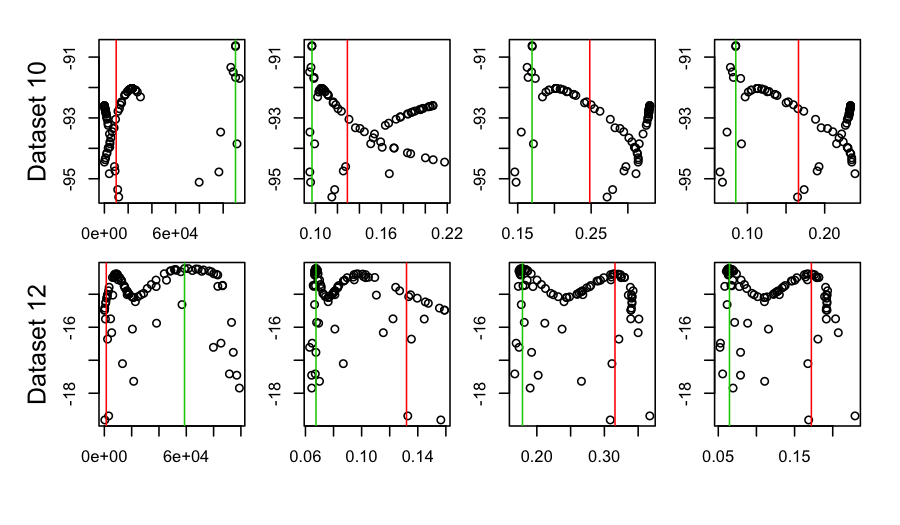
\includegraphics[width=\linewidth]{figure/lik-against-ests-2-1} \hfill{}

\caption[Plots of the likelihood against hte parameter estimates for some of the datasets reveals the existence of multiple likelihood peaks, one centered around a very high ]{Plots of the likelihood against hte parameter estimates for some of the datasets reveals the existence of multiple likelihood peaks, one centered around a very high $f_h$ value. When the likelihood is higher at this large $f_h$ peak, all of the other parameter estimates are pulled away from their true values.}\label{fig:lik-against-ests-2}
\end{figure}


\end{knitrout}

However, in Fig. \ref{fig:lik-against-ests-3}, you see cases where there are two peaks but the likelihood is higher at the peak with a low $f_h$ value.

\begin{knitrout}\scriptsize
\definecolor{shadecolor}{rgb}{0.969, 0.969, 0.969}\color{fgcolor}\begin{figure}

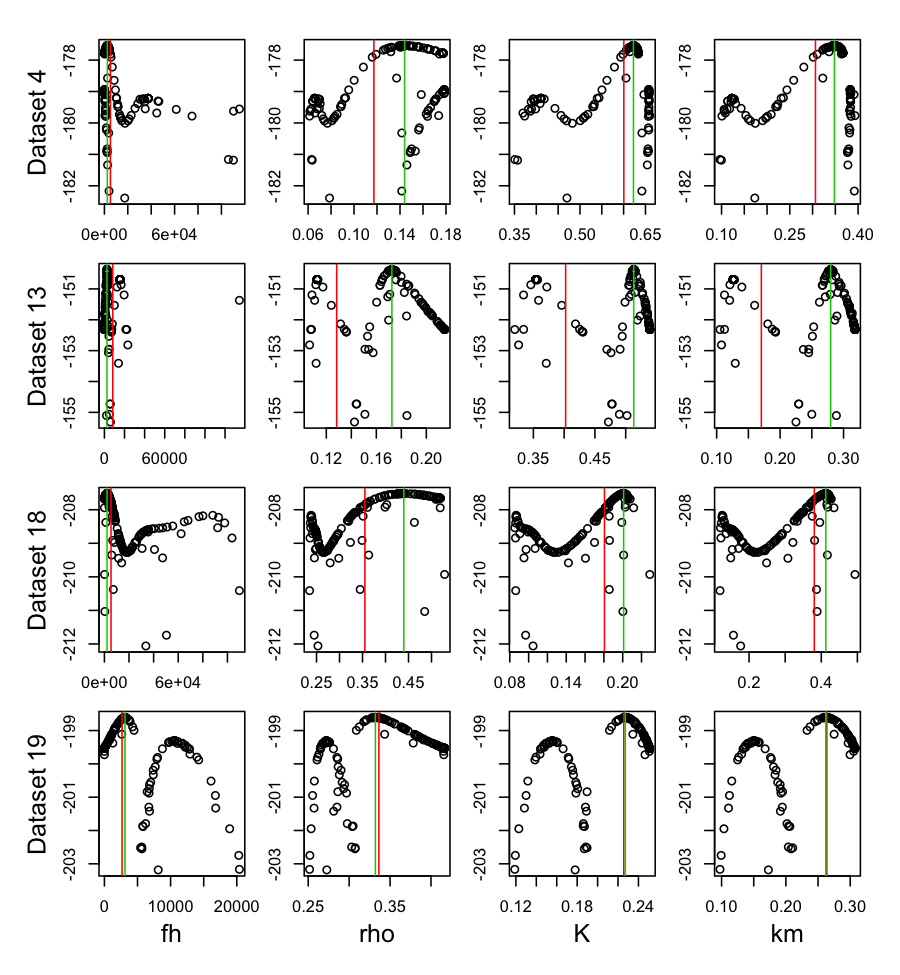
\includegraphics[width=\linewidth]{figure/lik-against-ests-3-1} \hfill{}

\caption[Plots of the likelihood against the parameter estimates for some of the datasets reveals the existence of multiple likelihood peaks]{Plots of the likelihood against the parameter estimates for some of the datasets reveals the existence of multiple likelihood peaks; in this case the likelihood is higher at the lower, more accurate, estimate.}\label{fig:lik-against-ests-3}
\end{figure}


\end{knitrout}

For still other datasets, the problem seems to be that the search algorithm got ``trapped'' at low values of $f_h$ (Fig. \ref{fig:lik-against-ests-4}).
It is possible that there was another peak in the likelihood surface at higher $f_h$ values that was never discovered by the fitting algorithm.

\begin{knitrout}\scriptsize
\definecolor{shadecolor}{rgb}{0.969, 0.969, 0.969}\color{fgcolor}\begin{figure}

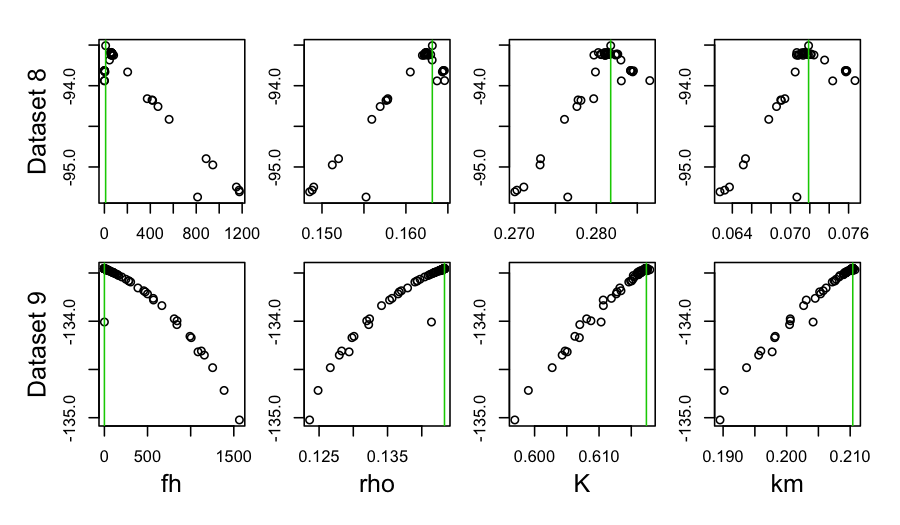
\includegraphics[width=\linewidth]{figure/lik-against-ests-4-1} \hfill{}

\caption[There were also datasets wherein the algorithm got stuck at low ]{There were also datasets wherein the algorithm got stuck at low $f_h$ values, never getting close to the truth.}\label{fig:lik-against-ests-4}
\end{figure}


\end{knitrout}

There were datasets that were simply hard to estimate, as evidenced by the fact that very few parameter sets had similar likelihoods (Fig. \ref{fig:lik-against-ests-5}).

\begin{knitrout}\scriptsize
\definecolor{shadecolor}{rgb}{0.969, 0.969, 0.969}\color{fgcolor}\begin{figure}

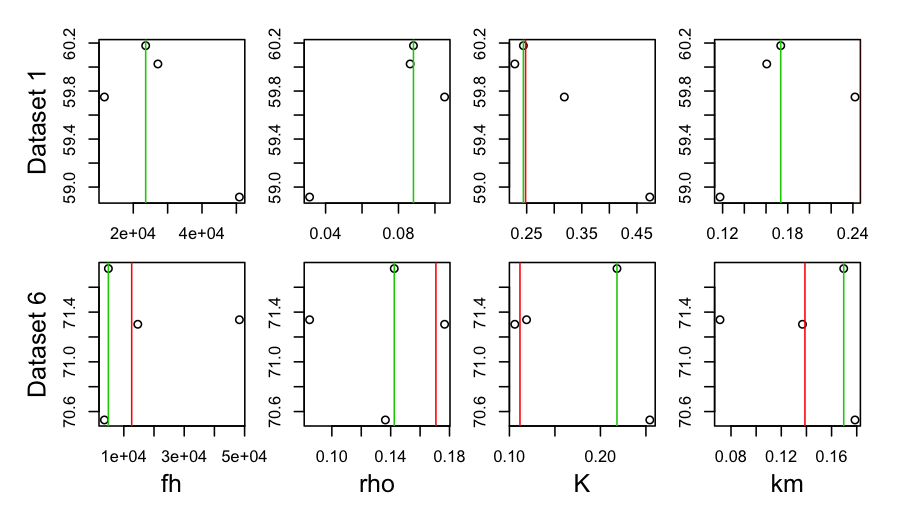
\includegraphics[width=\linewidth]{figure/lik-against-ests-5-1} \hfill{}

\caption[Some datasets were simply hard to estimate]{Some datasets were simply hard to estimate.}\label{fig:lik-against-ests-5}
\end{figure}


\end{knitrout}

\clearpage

However, if you compare the deterministic growth and reproduction trajectories at the true parameter values (red lines) to those trajectories at the best-fitting parameter set (black lines), you see that for all of the datasets, the best-fitting parameter set does a good job capturing the observed data (points).
You can see that, regardless of whether the parameter values were close to, or far from, the truth, the trajectories at the true and best-fitting parameters were always very close to one another.
The only things that you can conclude from looking at the fits is that datasets where growth is very slow and reproduction happens only at the end are very hard to fit, which is not surprising at all.
Otherwise, there doesn't really seem to be anything in the datasets themselves that separate the cases where the estimates were close from the cases where the estimates were far from the truth.
There is some limited evidence that very extreme datasets (e.g., when reproduction was exorbitant or very minimal) are harder to fit (e.g., datasets 3, 12, 18).

\begin{knitrout}\scriptsize
\definecolor{shadecolor}{rgb}{0.969, 0.969, 0.969}\color{fgcolor}\begin{figure}

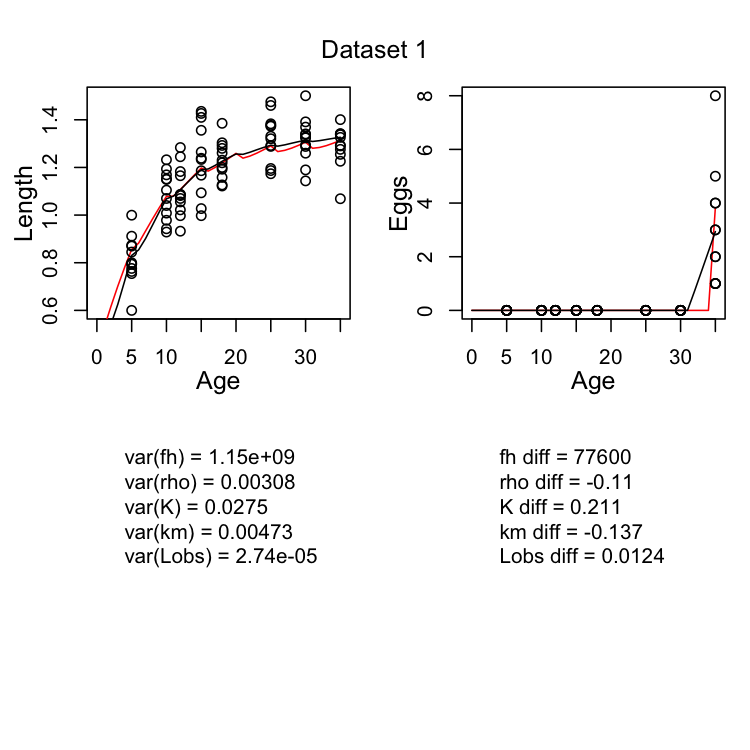
\includegraphics[width=0.6\textwidth]{figure/unnamed-chunk-4-1} \hfill{}

\caption[Plots of the raw observed length and egg data, along with the deterministic growth and reproduction trajectories at the true and best-fitting parameter sets]{Plots of the raw observed length and egg data, along with the deterministic growth and reproduction trajectories at the true and best-fitting parameter sets. Here we show those trajectories for parameter sets that were close to the truth.}\label{fig:unnamed-chunk-4}
\end{figure}


\end{knitrout}

\begin{knitrout}\scriptsize
\definecolor{shadecolor}{rgb}{0.969, 0.969, 0.969}\color{fgcolor}\begin{figure}

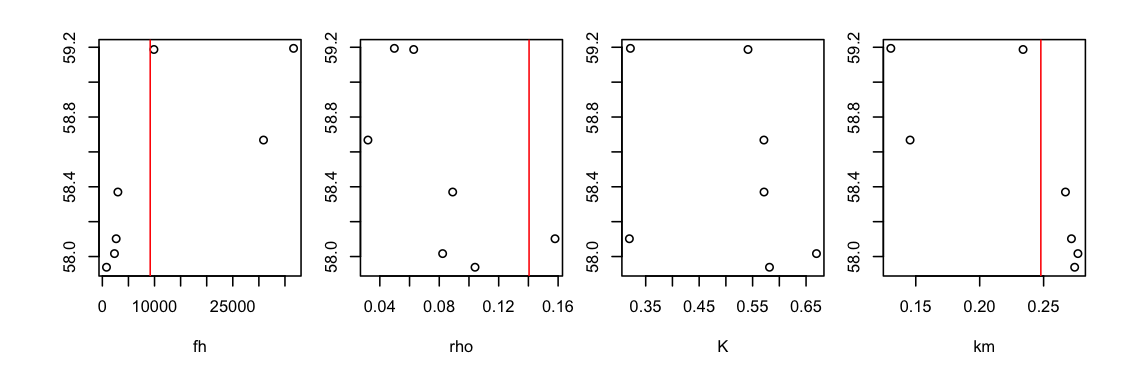
\includegraphics[width=0.6\textwidth]{figure/unnamed-chunk-5-1} \hfill{}

\caption[Plots of the raw observed length and egg data, along with the deterministic growth and reproduction trajectories at the true and best-fitting parameter sets]{Plots of the raw observed length and egg data, along with the deterministic growth and reproduction trajectories at the true and best-fitting parameter sets. Here are the trajectories for datasets that yielded two likelihood peaks and the best-fitting parameter set was far from the truth.}\label{fig:unnamed-chunk-5}
\end{figure}


\end{knitrout}

\begin{knitrout}\scriptsize
\definecolor{shadecolor}{rgb}{0.969, 0.969, 0.969}\color{fgcolor}\begin{figure}

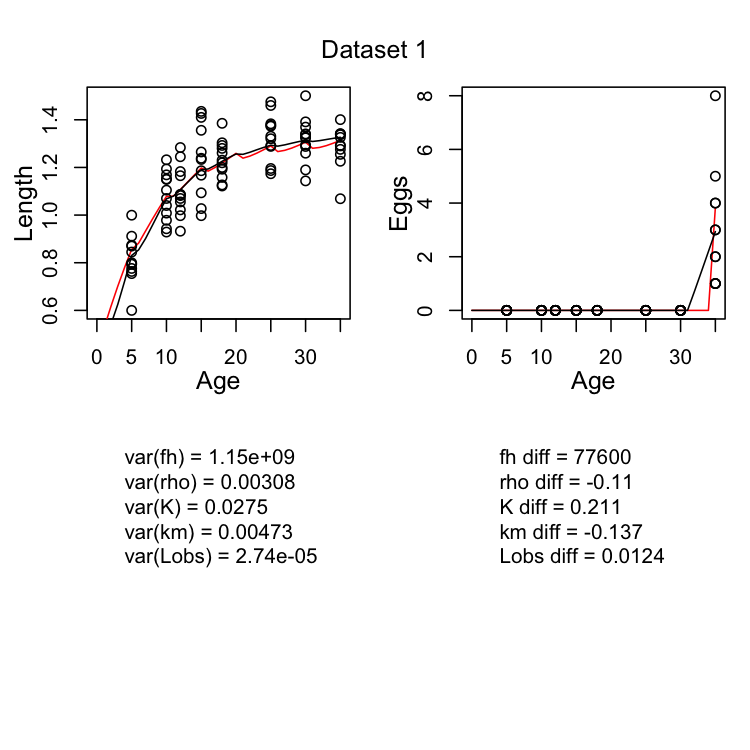
\includegraphics[width=0.6\textwidth]{figure/unnamed-chunk-6-1} \hfill{}

\caption[Plots of the raw observed length and egg data, along with the deterministic growth and reproduction trajectories at the true and best-fitting parameter sets]{Plots of the raw observed length and egg data, along with the deterministic growth and reproduction trajectories at the true and best-fitting parameter sets. Here are the trajectories for datasets that yielded two likelihood peaks and the best-fitting parameter set was closer to the truth.}\label{fig:unnamed-chunk-6}
\end{figure}


\end{knitrout}

\begin{knitrout}\scriptsize
\definecolor{shadecolor}{rgb}{0.969, 0.969, 0.969}\color{fgcolor}\begin{figure}

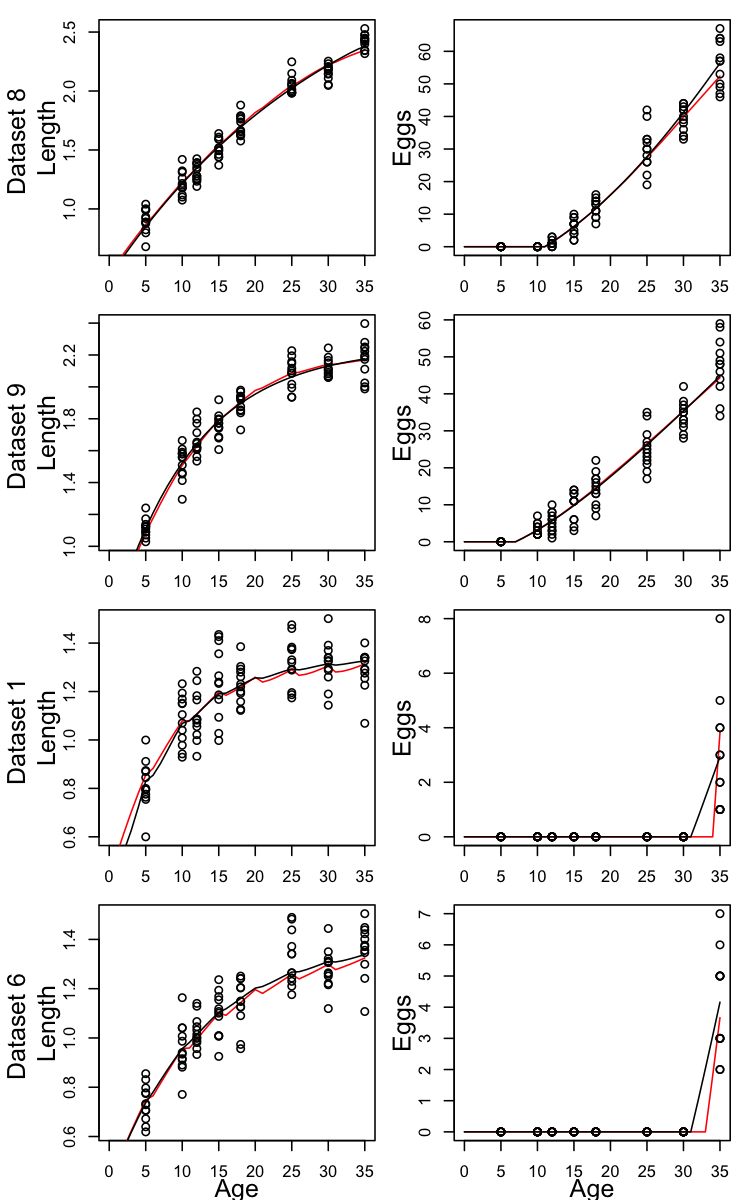
\includegraphics[width=0.6\textwidth]{figure/unnamed-chunk-7-1} \hfill{}

\caption[Plots of the raw observed length and egg data, along with the deterministic growth and reproduction trajectories at the true and best-fitting parameter sets]{Plots of the raw observed length and egg data, along with the deterministic growth and reproduction trajectories at the true and best-fitting parameter sets. Here are the trajectories when the parameter estimates got stuck at low $f_h$ values (8,9) or where the parameters were simply hard to estimate (1,6).}\label{fig:unnamed-chunk-7}
\end{figure}


\end{knitrout}


\clearpage

This suggests that it may not be possible to estimate all the parameters without error; it may be necessary to carry out profile likelihood calculations for $f_h$, in particular, to determine the topography of the likelihood surface along this direction.
However, we have some evidence that $\rho$, $\kappa$, and $k_m$ can all be estimated, so long as the other parameters related to feeding, length-biomass conversion, and the cost of reproduction are known.

\section*{Fitting the growth and reproduction trajectories of uninfected animals}
For this section, I need to use parameter values that make more sense for \emph{Daphnia dentifera}.
Hall et al. 2009 report that the mass of the host is $W=\alpha L^3$, where $\alpha=1.8\times 10^{-3}$ mgC mm$^{-3}$, and they assume (Appendix A) that half of the measured dry mass is carbon.
$L$ is the observed length, rather than the ``structural'' length of DEB theory; Spencer's formulation of the standard DEB model didn't involve the structural length, so this parameter wasn't needed.
In other words, $\alpha$ was estimated using observed dry weights $W$, observed lengths $L$, and an assumption that $W/2$ is the carbon mass of the host.

This is slightly different than what I am doing, but is not incompatible with it.
I had assumed that observed mass $W_{obs} = W + E$, where $W$ is the ``structural'' mass and $E$ is the reserves, and that observed length was $L_{obs} = \xi W_{obs}^q$, where $\xi$ and $q$ are based on a regression of observed weight on observed length.
I then assumed that ``structural length'' $L$ was equal to $W^{1/3}$.
So, basically, all I need to do is assume that $\xi=\alpha$ and $q=3$ and I will have recovered the same fitting.





I just discovered a big mistake in the code, so I need to redo some things - please oh please don't have that be a big deal!

\clearpage
\section*{Including parasitism}
I will include the structured model of parasitism into this model.
I will assume that the parasite shuts off reproduction by causing all energy allocated to reproduction to instead be allocated to growth.
I need to decide how the parasite uses this energy as a resource.

I will point out that castration is not instantaneous, as many individuals are able to have clutches (including clutches that are larger than normal) after exposure to the parasite.
We could assume that castration happens $n$ days post-infection, letting $n$ be estimated on the basis of the data.
However, in the data for Cat's experiments, castration precedes sexual maturity for all individuals, so it may be very difficult to estimate $n$.

How exactly the parasite uses energy from growth is trickier.
The total energy allocated to growth is $\kappa~E_G~p_C$ in DEB model (or just $p_C$ once castration happens).
Maintenance costs are subtracted from this total, and the remainder is used for growth, with a conversion cost of $E_G$.
The growth model (without parasitism) is just:
\begin{equation}
\frac{dV}{dt} = \frac{\kappa~p_C - k_m~E_G~V}{E_G}.
\end{equation}

There are several ways to incorporate parasite energy theft into growth.
Seemingly, the simplest is to assume that the parasite steals some fraction of the energy allocated to growth.
Focusing on the point after all energy is allocated towards growth (i.e., $\kappa=1$), we assume that the parasite steals some fraction $\sigma(N,E,V)$ of mobilized energy $p_C$. The remainder goes to fuel host growth. Then the model for growth and parasite population size (ignoring structure for simplicity) is something like:
\begin{align}
\frac{dV}{dt} &= \frac{(\kappa-\sigma(N,E,V))~p_C - k_m~E_G~V}{E_G}, \\
\frac{dN}{dt} &= \sigma(N,E,V)~p_C.
\end{align}
The fraction of energy stolen by the parasite could potentially depend on the number of parasites, the size of the host, the size of the host's energy reserves, or none of these things.
My results suggest that it might just be a constant fraction, regardless of the host's size or energetic state.
This result is problematic to interpret, given that my experiments did not keep track of immature spores.
However, if it was correct, then the total number of parasites would depend on the host and environmental factors that affect the mobilization flux $p_C$.
If the parasite population is structured, with multiple stages using energy, then figuring out exactly what fraction of the fraction of energy each stage gets is challenging.
The challenge is that $\sigma(N,E,V)$ becomes $\sigma(N_C, N_P, E, V)$, where it is the sum of the two parasite populations that affect how much total energy is stolen.
Given that this is a fraction, it must remain bounded between 0 and 1.
So, for example, if you have
\begin{equation}
\sigma = \frac{a_1 N_C + a_2 N_P}{1 + a_1 N_C + a_2 N_P},
\end{equation}
that ensures that the total fraction of energy stolen cannot be greater than one.

I think that simpler model would simply assume that the parasite utilizes structural bimoass as a resource.
In this case, we let $\sigma(N,V)$ be the parasite's rate of ``structure conversion to parasite biomass'' and the model for host and parasite growth becomes
\begin{align}
\frac{dV}{dt} &= \frac{\kappa~p_C - k_m~E_G~V }{E_G} - \sigma(N,V), \\
\frac{dN}{dt} &= \sigma(N,V).
\end{align}

More complicated are models where the parasite is utilizing energy that is allocated to growth in a dynamic way.
The reason this is slightly more complicated is that $\kappa~p_C$ is an energy flux; it has units of energy per time.
If we imagine the the parasite is acting as a ``predator'' on host energy, we would write down its ``functional response.''
For example, in Hall et al. 2009, Spencer had the parasite using energy reserves $E$ as a resource, and wrote down the parasite's per-capita growth rate as
\begin{equation}
a_N \frac{E}{h_N+E}-m_N.
\end{equation}
It is less obvious how to do that when the equivalent of $E$ in Hall et al. 2009 is $p_C$.
The simplest way is to simply treat $p_C$ as they did $E$.
That's fine (mathematically), but it is worth pointing out that the terms of this ``functional response'' don't have the same biological interpretation (and cannot be derived on the basis of a physical argument).
However, we will go with it for now, and say that $\sigma(N,p_C)$ is the functional response of the parasite.
There are two ways that the parasite might access energy.
\begin{align}
\frac{dV}{dt} &= \frac{\kappa~(p_C - \sigma(N,p_C)) - k_m~E_G~V}{E_G}, \\
\frac{dN}{dt} &= \sigma(N,p_C).
\end{align}
In this model, the parasite reduces the amount of mobilized energy available for growth.
The second model is
\begin{align}
\frac{dV}{dt} &= \frac{\kappa~p_C - k_m~E_G~V - \sigma(N,\kappa~p_C)}{E_G}, \\
\frac{dN}{dt} &= \sigma(N,p_C).
\end{align}
In this model, the parasite only has access to the energy that has been allocated to growth.
Of course, practically speaking, these two models will be identical because $\kappa=1$ once castration occurs.
So we can profitably reduce the number of models down to three by assuming that most (essentially, all) of the replication happens after castration has occurred.

I am also going to make an assumption that is not obvious here, which is that the mobilization rate rules do not change upon infection.
That is, the functional form of $p_C$ in infected hosts will be identical to that of uninfected hosts.
This is problematic is because the (admittedly obscure) derivation of the form of the mobilization rate equation relies on assumptions that are not met in infected hosts.
In particular, the DEB assumption of ``weak homeostasis'' is almost certainly violated.
This assumption states that, under constant food, there is a ``reserve density'' (defined by the quantity $E/V$) which remains constant.
Given that the parasite is developing inside the host, causing a rechanneling of energy and siphoning off some of that energy for itself, it seems very unlikely to imagine that the ratio of reserves to structure will remain constant.
However, previous work using DEB models to study infection (Hall et al. 2007, 2009 and Flye-Sainte-Marie et al. 2009) have not worried about violating this assumption, and those have been co-authored by DEB pioneers like Nisbet and Kooijman.
Thus, I will assume that this is not too big of a problem.

I am going to assume that the parasites hit structure for some simulation/recovery experiments.





\section*{Suggested future experiments}
Infection experiment with varying initiation of reduced food.
If I am correct that most (all) of the replication happens early in infection, then the total (transmission vs. pre-transmission) number of spores should be relatively unaffected by reductions in food late in infection.
However, the total number of transmission stages would be affected, because reducing the food late in infection reduces the developmental rate of the pre-transmission stages.
It also might increase density-dependent competition for resources.

another interesting thing would be to look at the adaptive value of anorexia.
Specifically, if you had several food treatments and you measured ingestion rates for sick and healthy individuals, and then compared fitnesses of individuals across treatments and within treatments against feeding depression.

\section*{Notes to self}

I also want to consider a ``net production'' model.
This model eliminates the need for a consideration of reserves.
Instead, we track the dynamics of total \emph{Daphnia} biomass.
Net production is calculated based on assimilation minus maintenance, which depends on biomass.
In this model, the parasite utilizes biomass as its resource.
Whether parasites increase or decrease host size depends on how much biomass is ``consumed'' by parasites and how much additional biomass is created by eliminating reproduction.
Previous studies have suggested that net production models might actually be a better fit to \emph{Daphnia} than net assimilation models anyway.

\subsection*{Derivation of the clearance model}
The clearance rate was calculated as $\log(F_0/F_T) (V/T)$, where $F_T$ is the final number of cells, $F_0$ is the initial number of cells, $V$ is the volume of the container, and $T$ is the amount of time the feeding trial lasted.
This comes from the following model of feeding (where $F(t)$ is the amount of food at any time $t$:
\begin{equation}
\frac{dF}{dt} = -a/V F(t)
\end{equation}
Implicit in this equation are the units of the parameters: $a$ is the clearance rate and has units of L/time; $V$ has units of L, and $F(t)$ has units of algal cells.
Solving and manipulating this equation:
\begin{align*}
&\frac{1}{F(t)} dF = -a/V dt \\
&\log(F(t)) = -at/V + C \\
&F(t) = F_0~e^{-at/V} \\
&F(T) = F_0~e^{-aT/V} \\
&e^{aT/V} = \frac{F_0}{F_T} \\
&\frac{aT}{V} = \log\left(\frac{F_0}{F_T}\right) \\
& a = \log\left(\frac{F_0}{F_T}\right) \left(\frac{V}{T}\right)
\end{align*}

\end{document}
